
%% tmm.tex
%% by Shengbin Meng

% Note that the a4paper option is mainly intended so that authors in
% countries using A4 can easily print to A4 and see how their papers will
% look in print - the typesetting of the document will not typically be
% affected with changes in paper size (but the bottom and side margins will).
% Use the testflow package mentioned above to verify correct handling of
% both paper sizes by the user's LaTeX system.
%
% Also note that the "draftcls" or "draftclsnofoot", not "draft", option 
% should be used if it is desired that the figures are to be displayed in
% draft mode.
%
\documentclass[journal,draftclsnofoot,onecolumn]{IEEEtran}
%\documentclass[journal]{IEEEtran}
%
% If IEEEtran.cls has not been installed into the LaTeX system files,
% manually specify the path to it like:
% \documentclass[journal]{../sty/IEEEtran}


 
% *** GRAPHICS RELATED PACKAGES ***
%
\ifCLASSINFOpdf
   \usepackage[pdftex]{graphicx}
  % declare the path(s) where your graphic files are
  % \graphicspath{{../pdf/}{../jpeg/}}
  % and their extensions so you won't have to specify these with
  % every instance of \includegraphics
   \DeclareGraphicsExtensions{.pdf,.jpeg,.png}
\else
  % or other class option (dvipsone, dvipdf, if not using dvips). graphicx
  % will default to the driver specified in the system graphics.cfg if no
  % driver is specified.
   \usepackage[dvips]{graphicx}
  % declare the path(s) where your graphic files are
  % \graphicspath{{../eps/}}
  % and their extensions so you won't have to specify these with
  % every instance of \includegraphics
   \DeclareGraphicsExtensions{.eps}
\fi
% graphicx was written by David Carlisle and Sebastian Rahtz. It is
% required if you want graphics, photos, etc. graphicx.sty is already
% installed on most LaTeX systems. The latest version and documentation
% can be obtained at: 
% http://www.ctan.org/tex-archive/macros/latex/required/graphics/
% Another good source of documentation is "Using Imported Graphics in
% LaTeX2e" by Keith Reckdahl which can be found at:
% http://www.ctan.org/tex-archive/info/epslatex/
%
% latex, and pdflatex in dvi mode, support graphics in encapsulated
% postscript (.eps) format. pdflatex in pdf mode supports graphics
% in .pdf, .jpeg, .png and .mps (metapost) formats. Users should ensure
% that all non-photo figures use a vector format (.eps, .pdf, .mps) and
% not a bitmapped formats (.jpeg, .png). IEEE frowns on bitmapped formats
% which can result in "jaggedy"/blurry rendering of lines and letters as
% well as large increases in file sizes.
%
% You can find documentation about the pdfTeX application at:
% http://www.tug.org/applications/pdftex


% *** MATH PACKAGES ***
%
\usepackage[cmex10]{amsmath}
% A popular package from the American Mathematical Society that provides
% many useful and powerful commands for dealing with mathematics. If using
% it, be sure to load this package with the cmex10 option to ensure that
% only type 1 fonts will utilized at all point sizes. Without this option,
% it is possible that some math symbols, particularly those within
% footnotes, will be rendered in bitmap form which will result in a
% document that can not be IEEE Xplore compliant!
%
% Also, note that the amsmath package sets \interdisplaylinepenalty to 10000
% thus preventing page breaks from occurring within multiline equations. Use:
%\interdisplaylinepenalty=2500
% after loading amsmath to restore such page breaks as IEEEtran.cls normally
% does. amsmath.sty is already installed on most LaTeX systems. The latest
% version and documentation can be obtained at:
% http://www.ctan.org/tex-archive/macros/latex/required/amslatex/math/


% *** ALIGNMENT PACKAGES ***
%
\usepackage{array}
% Frank Mittelbach's and David Carlisle's array.sty patches and improves
% the standard LaTeX2e array and tabular environments to provide better
% appearance and additional user controls. As the default LaTeX2e table
% generation code is lacking to the point of almost being broken with
% respect to the quality of the end results, all users are strongly
% advised to use an enhanced (at the very least that provided by array.sty)
% set of table tools. array.sty is already installed on most systems. The
% latest version and documentation can be obtained at:
% http://www.ctan.org/tex-archive/macros/latex/required/tools/


% *** SPECIALIZED LIST PACKAGES ***
%
\usepackage{algorithmic}
% algorithmic.sty was written by Peter Williams and Rogerio Brito.
% This package provides an algorithmic environment fo describing algorithms.
% You can use the algorithmic environment in-text or within a figure
% environment to provide for a floating algorithm. Do NOT use the algorithm
% floating environment provided by algorithm.sty (by the same authors) or
% algorithm2e.sty (by Christophe Fiorio) as IEEE does not use dedicated
% algorithm float types and packages that provide these will not provide
% correct IEEE style captions. The latest version and documentation of
% algorithmic.sty can be obtained at:
% http://www.ctan.org/tex-archive/macros/latex/contrib/algorithms/
% There is also a support site at:
% http://algorithms.berlios.de/index.html
% Also of interest may be the (relatively newer and more customizable)
% algorithmicx.sty package by Szasz Janos:
% http://www.ctan.org/tex-archive/macros/latex/contrib/algorithmicx/

% *** PDF, URL AND HYPERLINK PACKAGES ***
%
\usepackage{url}
% url.sty was written by Donald Arseneau. It provides better support for
% handling and breaking URLs. url.sty is already installed on most LaTeX
% systems. The latest version and documentation can be obtained at:
% http://www.ctan.org/tex-archive/macros/latex/contrib/url/
% Basically, \url{my_url_here}.


% *** Do not adjust lengths that control margins, column widths, etc. ***
% *** Do not use packages that alter fonts (such as pslatex).         ***
% There should be no need to do such things with IEEEtran.cls V1.6 and later.
% (Unless specifically asked to do so by the journal or conference you plan
% to submit to, of course. )


% correct bad hyphenation here
\hyphenation{op-tical net-works semi-conduc-tor}

% added by shengbin
\usepackage{verbatim}
\usepackage{multirow}
\usepackage{subfig}
\usepackage{algorithm}
\usepackage{balance}
\usepackage{makecell}


% paper title
% can use linebreaks \\ within to get better formatting as desired
% Do not put math or special symbols in the title.
\title{Adaptive Video Streaming with Optimized Bitstream Extraction and PID-based Quality Control}

% author names and IEEE memberships
% note positions of commas and nonbreaking spaces ( ~ ) LaTeX will not break
% a structure at a ~ so this keeps an author's name from being broken across
% two lines.
% use \thanks{} to gain access to the first footnote area
% a separate \thanks must be used for each paragraph as LaTeX2e's \thanks
% was not built to handle multiple paragraphs
%
\author{Shengbin~Meng, Jun~Sun, {\em Member, IEEE}, Yizhou~Duan and Zongming~Guo, {\em Member, IEEE} % <-this % stops a space
\thanks{Manuscript received July 15, 2015; revised December 3, 2015 and January 12, 2016; accepted February 21, 2016. This work was supported by  National Key Technology R\&D Program of China under Grant 2015AA011605 and National Natural Science Foundation of China under contract No. 61271020.}
\thanks{Copyright (c) 2013 IEEE. Personal use of this material is permitted. However, permission to use this material for any other purposes must be obtained from the IEEE by sending a request to pubs-permissions@ieee.org.}
\thanks{The authors are with the Institute of Computer Science and Technology, Peking University, Beijing%
, 100080, China (email: mengshengbin@pku.edu.cn, sunjun@pku.edu.cn, duanyizhou@pku.edu.cn, guozongming@pku.edu.cn). Jun Sun and Zongming Guo are also with the Cooperative Medianet Innovation Center, Shanghai, 200240, China. Jun Sun is the corresponding author.}
}

% note the % following the last \IEEEmembership and also \thanks - 
% these prevent an unwanted space from occurring between the last author name
% and the end of the author line. i.e., if you had this:
% 
% \author{....lastname \thanks{...} \thanks{...} }
%                     ^------------^------------^----Do not want these spaces!
%
% a space would be appended to the last name and could cause every name on that
% line to be shifted left slightly. This is one of those "LaTeX things". For
% instance, "\textbf{A} \textbf{B}" will typeset as "A B" not "AB". To get
% "AB" then you have to do: "\textbf{A}\textbf{B}"
% \thanks is no different in this regard, so shield the last } of each \thanks
% that ends a line with a % and do not let a space in before the next \thanks.
% Spaces after \IEEEmembership other than the last one are OK (and needed) as
% you are supposed to have spaces between the names. For what it is worth,
% this is a minor point as most people would not even notice if the said evil
% space somehow managed to creep in.



% The paper headers
%\markboth{IEEE TRANSACTIONS ON CIRCUITS AND SYSTEMS FOR VIDEO TECHNOLOGY,~Vol.~11, No.~4, December~2013}%
%{Shengbin Meng \MakeLowercase{\textit{et al.}}: Efficient H.264/SVC Bitstream Extraction Based on a Linear Error Model}
% The only time the second header will appear is for the odd numbered pages
% after the title page when using the twoside option.
% 
% *** Note that you probably will NOT want to include the author's ***
% *** name in the headers of peer review papers.                   ***
% You can use \ifCLASSOPTIONpeerreview for conditional compilation here if
% you desire.




% If you want to put a publisher's ID mark on the page you can do it like
% this:
%\IEEEpubid{0000--0000/00\$00.00~\copyright~2012 IEEE}
% Remember, if you use this you must call \IEEEpubidadjcol in the second
% column for its text to clear the IEEEpubid mark.



% use for special paper notices
%\IEEEspecialpapernotice{(Invited Paper)}



\begin{document}

%\listoffigures

%\listoftables


% make the title area
\maketitle

% As a general rule, do not put math, special symbols or citations
% in the abstract or keywords.
\begin{abstract}
To cope with the challenges brought about by bandwidth fluctuation and improve the experience of watching online videos, an adaptive video streaming system that can adjust video quality according to actual network conditions is proposed based on the Scalable Video Coding (SVC) extension of H.264/AVC. First, a simple and effective linear error model is proposed and verified for quality scalability of SVC. The model exploits the linear feature of pixel value errors and can be used to accurately estimate the distortion caused by discarding any combination of enhancement data packets in an SVC bitstream. On that basis, a greedy-like algorithm is designed to assign each data packet a priority value according to its Rate-Distortion (R-D) impact, thus enabling R-D optimized bitstream extraction under certain bitrate constraints. Finally, the Proportional-Integral-Derivative (PID) method is utilized to control the video quality adjustment and determine a suitable bitrate for transmission. By monitoring and predicting past, current and future bandwidth information, the PID-based quality control algorithm is able to reduce quality fluctuation while still preserving a high quality level. Experimental results show that compared with the baseline software, the proposed system that integrates the above algorithms can achieve much lower video quality fluctuation, with PSNR variance reduced from 1.24 to 0.69, and at the same time deliver higher video quality, with the PSNR average increased by 0.83 dB.
\end{abstract}

% Note that keywords are not normally used for peerreview papers.
\begin{IEEEkeywords}
video streaming, quality control, bitstream extraction, distortion model, Scalable Video Coding, PID.
\end{IEEEkeywords}



% For peer review papers, you can put extra information on the cover
% page as needed:
% \ifCLASSOPTIONpeerreview
% \begin{center} \bfseries EDICS Category: 3-BBND \end{center}
% \fi
%
% For peerreview papers, this IEEEtran command inserts a page break and
% creates the second title. It will be ignored for other modes.
\IEEEpeerreviewmaketitle



\section{Introduction}
\label{sec:intro}
% The very first letter is a 2 line initial drop letter followed
% by the rest of the first word in caps.
% 
% form to use if the first word consists of a single letter:
% \IEEEPARstart{A}{demo} file is ....
% 
% form to use if you need the single drop letter followed by
% normal text (unknown if ever used by IEEE):
% \IEEEPARstart{A}{}demo file is ....
% 
% Some journals put the first two words in caps:
% \IEEEPARstart{T}{his demo} file is ....
% 
\IEEEPARstart{V}{ideo} streaming applications are becoming more and more popular on the Internet. Examples of the most common usage scenarios are Video-on-Demand (VoD), live broadcasting, video-based online education, etc. In these applications, video data are constantly delivered to different clients over various transmission channels, and the client media player can begin to play the video before the entire file has been transmitted. Among other features, video streaming makes it easy to watch videos anywhere and anytime, which represents the concept of Ubiquitous Multimedia Access (UMA), a very common topic within the multimedia community \cite{Gualdi08}. Due to its convenience, video streaming also attracts a large number of users and has become an increasingly important way for people to consume video content \cite{Chen13}.

In video streaming, the network conditions significantly influence the user's watching experience. To provide better network conditions, some researchers choose to adopt the new Software Defined Networking (SDN) architecture \cite{Egilmez14}. Based on a successful SDN paradigm named OpenFlow, noticeable results are achieved. For instance, a solution for improving throughput in hybrid networks is proposed in \cite{Li14} and a demonstration of OpenFlow-controlled network orchestration for video manycast is presented in \cite{Xue15}. Although these studies have offered a promising way to optimize network conditions, traditional best-effort networks still dominate currently, and the variety of user network environments remains to be one of the biggest challenges for video streaming. A user may use different types of networks (Ethernet, Wi-Fi, Cellular, etc) and may also switch from one type to another on going (e.g., from Wi-Fi to Cellular). Even in the same network, the end-to-end bandwidth will change from time to time, influenced by the overall traffic. Within such an environment, bandwidth fluctuation is inevitable, and it would be difficult or impossible for the user to get best watching experience if the video is streamed at a fixed bitrate. To cope with this challenge, the video streaming system should be able to adjust the video's bitrate or quality according to the network condition. In other words, the video streaming system needs to be adaptive.

There are generally two options for enabling adaptive video streaming. The first option is called simulcast, where several independent bitstreams, each with different video quality, are stored at the server, and the client selects one of them according to the currently available bandwidth. Dynamic Adaptive Streaming over HTTP (DASH) \cite{DASH}, which is standardized by the Moving Picture Expert Group (MPEG), belongs to this option. The second option is to adopt the Scalable Video Coding (SVC) \cite{SVC} technology, an extension of the H.264/AVC video coding standard \cite{SVCOverview}, which allows scalability of video quality and bitrate with only one single bitstream. In SVC, a video bitstream is composed of small data packets called Network Abstract Layer Units (NALUs). These NALUs are separated into one base layer for basic video quality and multiple enhancement layers for video quality improvement. By discarding the NALUs of the enhancement layers, the bitstream can be extracted to provide the most appropriate video quality and bitrate as required.

Due to their easy deployment \cite{Bouten14}, simulcast systems are already used by many commercial video websites (e.g., YouTube \cite{YouTube}) to enable quality adaptation. However, the adaptive range and granularity that simulcast provides is limited to the number of streams (YouTube videos have 5 quality levels at most: 240p, 360p, 480p, 720p and 1080p), and the processing and storage of multiple video streams require large amounts of computation time and disk space. In order to provide a wide range of seamless quality adaptation at reasonable time and space cost, the adoption of SVC is necessary. An SVC video bitstream can be extracted at the fine granularity of one NALU (a very small partition of data), and performance analysis \cite{SVCPerformance} shows that SVC also has much higher coding efficiency than simulcast, where the same content is encoded multiple times. Therefore, adopting SVC in the video streaming framework is technically a better option and has attracted a lot of attention in the academia \cite{Chuah12}-\cite{Cicalo14}.

While these studies mostly focus on Quality of Service (QoS) optimization and resource allocation for specific networks, there are two key problems that need to be primarily addressed in the SVC adaptive video streaming system. First, as a prerequisite for bitrate adaption, the whole bitstream needs to be extracted so that sub-streams with various bitrates can be obtained. This is called the bitstream extraction problem. Optimal bitstream extraction algorithm aims to extract a sub-stream with the best video quality, or minimal distortion, under the constraint of a given bitrate. Second, when the bandwidth changes with time, it is necessary to make decisions about whether and how to adjust the video quality or bitrate. This problem is called quality control, which means controlling the video quality (or the bitrate, from the transmission point of view) to follow the change of the bandwidth. A good quality control algorithm should determine a suitable bitrate according to current network conditions, and maintain the video quality to be both smooth and at a high level.

In this paper, an efficient adaptive video streaming system based on SVC is proposed with the above two problems better solved. Apple Darwin Streaming Server (DSS) \cite{DSS}, which is open-sourced and has been widely used to stream multimedia content in practice, is chosen as the basis for the proposed system. The original DSS project is modified and SVC support is added to it for the purpose of both research and application. Novel algorithms for bitstream extraction and quality control are then designed and implemented to enable better quality of service for the user. The contributions of our work can be summarized as follows:
\begin{itemize}
\item First, a simple and effective Linear Error Model (LEM) is proposed and verified, which can be used to accurately estimate the distortion caused by discarding any combination of data packets from an SVC bitstream.
\item Second, utilizing distortion estimation with LEM, a greedy-like algorithm is designed to assign priority for each data packet according to its Rate-Distortion (R-D) impact, thus enabling optimized bitstream extraction.
\item Finally, for the quality control problem, a novel algorithm based on the Proportional-Integral-Derivative (PID) controller is proposed to replace the native one in DSS, and much lower quality fluctuation is achieved.
\end{itemize}

The proposed solutions for bitstream extraction and quality control are combined together and result in a higher and smoother PSNR curve representing the final video quality delivered to the user.

The rest of this paper is organized as follows. In section \ref{sec:analysis}, we analyze the problems in detail and introduce some related work on them. Then in section \ref{sec:bitstream-extraction}, the linear error model and the solution for the bitstream extraction problem are presented. The PID-based quality control algorithm is proposed in section \ref{sec:quality-control}. Section \ref{sec:experiment} lists the experimental results and compares our proposed solution with others. Finally, in section \ref{sec:conclusion}, we conclude this paper and point out related future work.


%%%%%%%%%%%%%%%%%%%%%%%%%%%%%%%%%%%%%%%%%%%%%%%%%%%%%%%%%%%%%
\section{Problem Analysis and Related Work}
\label{sec:analysis}

In this section, we analyze the two most important problems in SVC adaptive video streaming, i.e., bitstream extraction and quality control, and introduce some related work on them.

\subsection{Bitstream Extraction}
\label{subsec:analysis-extraction}

Bitstream extraction is the operation of choosing a subset of data packets from a whole SVC bitstream to form a sub-stream. Fig. \ref{fig:Bitstream-Extraction} illustrates the structure of an SVC bitstream and a possible way of extracting a sub-stream from it. The data packets in the bitstream are divided into different layers. The temporal layer (T0$\sim$T3) reflects the reference or dependency relationship between the frames. The arrows ot the top point from the referenced frame to the frame which is dependent on it. The quality layer (Q0$\sim$Q2) indicates the scalability of the video quality within each frame. Data packets in the higher quality layers (i.e., Q1 and Q2) are partially discarded to implement the extraction. For example, the dashed line demonstrates the extraction which will keep the data packets below the line and discard all the packets above it.

\begin{figure}[h]
\centering
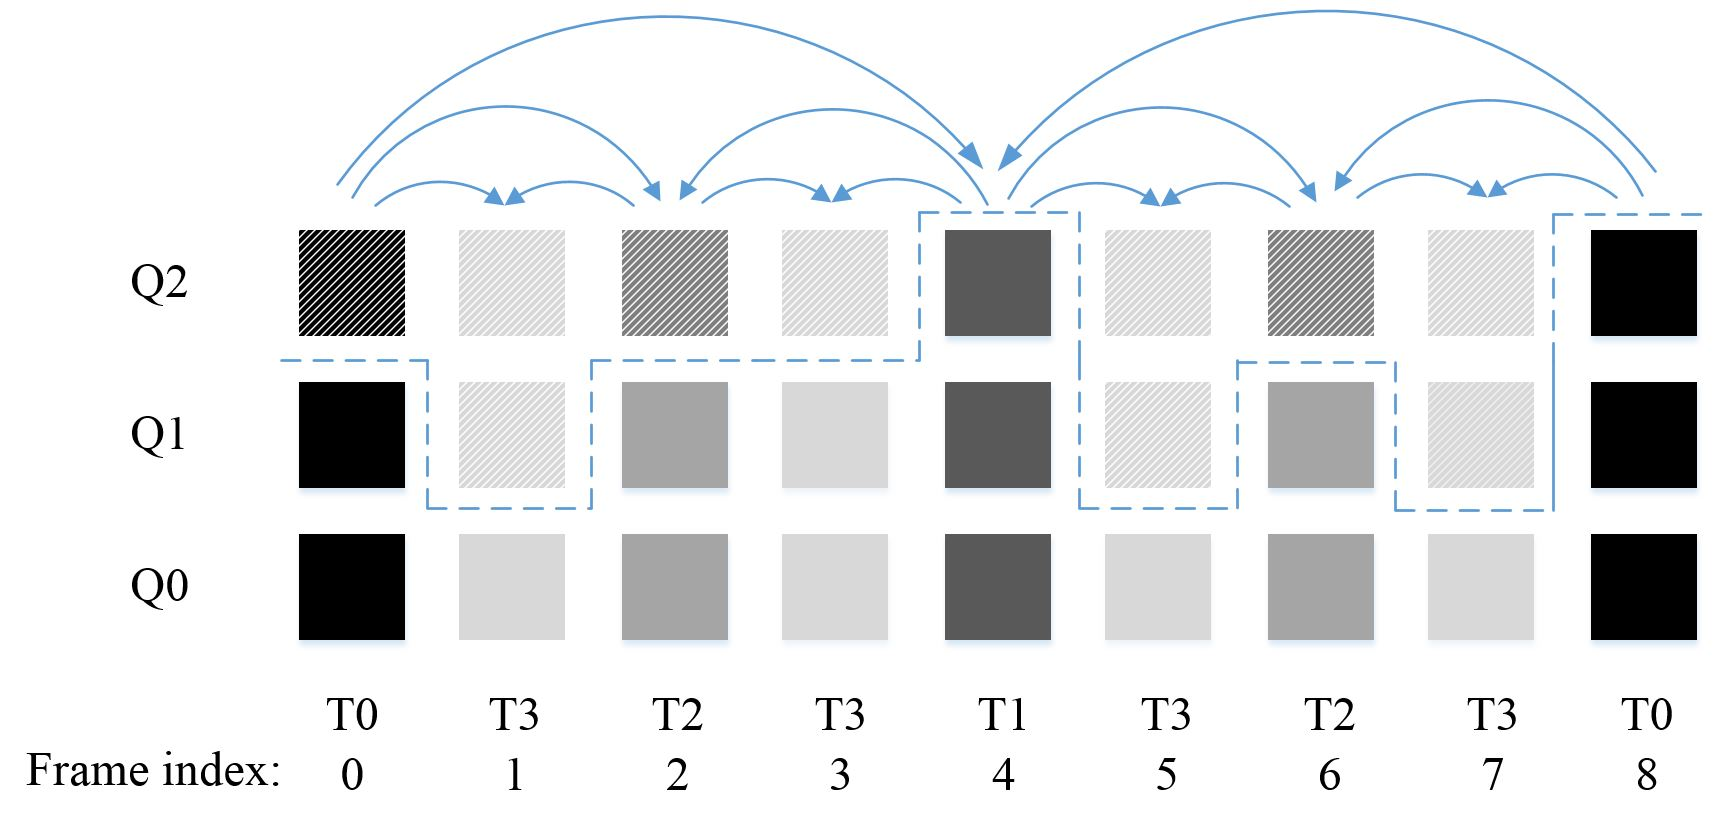
\includegraphics[width = 0.9\linewidth]{Bitstream-Extraction.jpg}
\caption{Bitstream extraction of SVC \label{fig:Bitstream-Extraction}}
\end{figure}

As we can see, in its nature SVC bitstream extraction is a combinatorial optimization problem. There are many combinations of packets to be discarded, and we want to choose a combination that maximizes the video quality of the extracted sub-stream, under the constraint of a given bitrate. More specifically, this problem is in the form of the ``0-1 Knapsack Problem" \cite{Knapsack}. Each data packet can be treated as an object with certain weight (the packet's size) and value (its contribution to the video quality). The solving process is mainly deciding whether or not a packet should be included in the final extracted sub-stream, or, in terms of the ``0-1 Knapsack Problem", choosing which object to pack up.

For a typical ``0-1 Knapsack Problem", the optimal solution can generally be found using the dynamic programming algorithm. However, this is not operational for the bitstream extraction problem, mainly due to the dependence between the data packets. First, the subset of packets to be extracted cannot be chosen arbitrarily, because if a packet is included, all the packets it depends on must also be included. For example, in Fig. \ref{fig:Bitstream-Extraction}, we cannot include the Q2 packet of a frame without including the Q1 packet of the same frame. Second, the value of a packet is not obvious and certain, because a packet's contribution to video quality depends on other packets and may vary for different extractions. There is no way to exactly determine the video quality of an extracted sub-stream, unless we perform the extraction and calculate the distortion for real. To the best of our knowledge, no method presented in the literature claims to find the optimal solution of the SVC bitstream extraction problem. All the efforts are made to obtain a solution that is as good as possible.

In \cite{Amonou07}, Amonou et al. proposed a bitstream extraction framework based on the concept of \textit{Quality Layers}. This framework has been adopted by the SVC reference software, i.e., JSVM \cite{JSVM}, and achieves better R-D performance compared to the basic extractor of JSVM. In Amonou's framework, a Quality Layer value, which reflects a data packet's R-D impact, is calculated and used for R-D optimized bitstream extraction. The process of obtaining the distortion impact of every packet is extremely time consuming, and the distortion estimation accuracy can also be further improved. Therefore, other distortion/error models were proposed to either reduce the computational complexity or improve the estimation accuracy. Sun et al. \cite{Sun09} and Maani et al. \cite{Maani09} constructed models to calculate the distortion based on the drift propagation between frames. Sun et al.'s method is almost as good as JSVM in terms of performance, but has much reduced complexity. Maani et al.'s model can achieve better estimation accuracy than JSVM; however, since it is a training-based model, more computation is needed to get robust model parameters. Ramanathan et al. \cite{Ramanathan12} proposed their concept and calculation method of the ``Quality Metadata'' to signal and use in bitstream extraction. Yang et al. \cite{Yang13} proposed a method based on simulated annealing to solve the bitstream extraction problem. In both methods, the accuracy of distortion estimation affects the performance significantly. With an accurate estimation of a packet's distortion impact, its prioritization order during extraction can be determined. A priority value can then be assigned to it and stored in the bitstream for optimized extraction in the future. In \cite{Lim06}, Lim et al. treated the SVC bitstream as a tree structure and assigned extraction priority accordingly. In \cite{Zhu11}, Zhu et al. chose to assign priority values derived using the Langrange multiplier method.

In our previous work \cite{Zhang12}, we proposed a linear error model for distortion estimation and priority assignment, based on which good bitstream extraction performance is achieved. However, this work assumes that the original video sequence is available for reference, which is not always true. How to handle the special characteristic of the no-reference case is lacking in the previous work and included in this paper.

\subsection{Quality Control}
\label{subsec:analysis-control}

Quality control is the second problem we will address in this paper. A quality control algorithm gives the suitable bitrate for transmission, which is directly related to the change of the video quality delivered to the user. In an SVC streaming system, the bitrate determined by the quality control algorithm is used as the constraint under which bitstream extraction is performed. Even in non-SVC streaming systems (DASH, for example), quality control is an important aspect that requires careful design.

For a quality control algorithm, there are three targets to be achieved. The first is ensuring the continuity of video play. In real-time streaming systems, each data packet has its own playtime, which is also treated as the deadline of the transmission. If the packet does not arrive at the client side before the deadline, the media player will be paused due to lack of data, and that should be avoided. The second is maintaining smooth video quality. Although network conditions may change rapidly, it is necessary for the streamed video to maintain a relatively stable quality level, because frequent change of video quality will lead to poor user experience. The third target is to make the video quality as good as possible. In other words, the available bandwidth should be fully utilized. Suppose we keep sending video data at a low bitrate (with low video quality), neither will the playback pause nor will any quality fluctuation occur. However, a low video quality is certainly not what the user wants.

The state-of-the-art solutions for avoiding playback pause in the client media player mainly focus on how to select and schedule the video packets. In \cite{Gao06}, K. Gao et al. proposed a priority-based scheduling strategy, which guarantees that packets of higher importance will be transmitted earlier. Among the packets with the same priority, those with the earliest deadline will be transmitted first. A similar solution is proposed in \cite{Schierl10}, where the video data are pre-buffered in several buffers of different priorities. Whenever re-buffering occurs, the quality will be degraded to a lower level to meet the time and rate constraints. Although the priority-based scheduling strategies perform well in maintaining a non-paused video play, they do not take quality fluctuation into account. As a result, users may still suffer from the frequent fluctuation of video quality.

In the widely used video streaming server DSS, quality control is implemented by monitoring packet delay (the difference between the current time and the playing time of this packet). When a new packet is ready to be sent to the streaming buffer, DSS checks its delay and compares this delay with some pre-set thresholds to judge whether a quality change should be made and how extreme it should be. This algorithm can reduce quality fluctuation to some degree. However, it only provides conservative quality changes, which makes its reaction so slow that sometimes the media player may have already stopped due to lack of video data before the quality drops. Furthermore, this algorithm does not keep track of the bandwidth change, and therefore, it can only adjust the video quality based on the current state. Quality oscillation might occur in this algorithm.

In the following part of this paper, we will present our solution for each of the problems. The solutions then work in combination and serve as a solid foundation for a practical adaptive video streaming system. It should be noted that in practical streaming systems, another issue of concern is the occasional packet loss during transmission, which will cause decoding errors and corrupted images, resulting in a significant degradation of video quality. Avoiding or even recovering from packet loss/error is an important research topic that is popular in both the networking and multimedia communities. However, in this paper, which focuses on server-side adaptation, packet loss is not handled, and the video stream is assumed to be successfully delivered to the client.

%%%%%%%%%%%%%%%%%%%%%%%%%%%%%%%%%%%%%%%%%%%%%%%%%%%%%%%%%%%%%
\section{Optimized Bitstream Extraction Based on Linear Error Model}
\label{sec:bitstream-extraction}

Being able to adjust the bitrate is the prerequisite of an adaptive video streaming system. For SVC videos, this means extracting a subset of packets from the whole bitstream. How to optimally choose this subset to achieve minimum distortion under the given bitrate is the key point of the bitstream extraction problem. In this section, we propose a linear error model and a greedy-like algorithm to solve this problem.

\subsection{Linear Error Model for Quality Scalable Video}
\label{subsec:linear-model}

In H.264/AVC, the decoding process involves a linear feature described in \cite{Winken08}. According to this feature, the main steps of decoding -- prediction, transform and quantization -- are approximately linear operations (neglecting any rounding, clipping, and deblocking filtering), and the whole process can be expressed in a matrix format as follows:
\begin{equation}
\label{eq:linear}
s = {\rm\bf M} \cdot s + {\rm\bf T} \cdot c + p \: .
\end{equation}
It means, the reconstructed samples of a Group of Pictures (GOP), denoted by $s$, can be viewed as a linear combination of previously reconstructed samples in the GOP, the residuals, and a static predictor. In (\ref{eq:linear}), $c$ refers to the transform coefficients, and $p$ is a static predictor; ${\rm\bf M}$ and ${\rm\bf T}$ are square matrices such that ${\rm\bf M} \cdot s$ gives the Motion Compensated Prediction (MCP) signal and ${\rm\bf T} \cdot c$ gives the residuals. The actual values of ${\rm\bf M}$ depend on the selected macroblock types, reference indices and motion vectors, whereas the actual values of ${\rm\bf T}$ depend on the chosen Quantization Parameter (QP).

We apply the above linear decoding feature to the case of quality scalability of SVC and obtain a Linear Error Model (LEM). According to (\ref{eq:linear}), for a bitstream just containing the base layer, we have:
\begin{equation}
\label{eq:base0}
s_{B} = {\rm\bf M} \cdot s_{B} + {\rm\bf T}_{B} \cdot c_{B} + p \: ,
\end{equation}
where the subscript $B$ indicates the base layer variables. In quality scalability, the enhancement is mainly the refinement of the transform coefficients. For a bitstream containing an enhancement packet set $I_1$, the reconstruction relationship can be expressed as:
\begin{equation}
\label{eq:subset1}
s_{I_1} = {\rm\bf M} \cdot s_{I_1} + {\rm\bf T}_{B} \cdot c_{B} + \Big( \sum_{i \in I_1}{\rm\bf T}_i \cdot c_i \Big) + p \: ,
\end{equation}
where $i$ refers to an enhancement packet in the set $I_1$, $c_i$ is a vector containing coefficients within the enhancement packet $i$, ${\rm\bf T_i}$ is the transform matrix depending on the QP value of $i$ and ${\rm\bf T}_i \cdot c_i$ gives the residual values decoded from $i$.

Similarly, for another bitstream containing an enhancement packet set $I_2$, we have
\begin{equation}
\label{eq:subset2}
s_{I_2} = {\rm\bf M} \cdot s_{I_2} + {\rm\bf T}_{B} \cdot c_{B} + \Big( \sum_{i \in I_2}{\rm\bf T}_i \cdot c_i \Big) + p \: .
\end{equation}

If $I_1$ is a subset of $I_2$, their reconstruction difference can be obtained by (\ref{eq:subset2}) - (\ref{eq:subset1}):
\begin{equation}
\label{eq:minus1}
(s_{I_2} - s_{I_1}) = {\rm\bf M} \cdot (s_{I_2} - s_{I_1}) + \Big( \sum_{i \in I_2}{\rm\bf T}_i \cdot c_i - \sum_{i \in I_1}{\rm\bf T}_i \cdot c_i \Big) \: ,
\end{equation}
\begin{equation}
\label{eq:minus2}
\Rightarrow e = s_{I_2} - s_{I_1} = ({\rm\bf I - M})^{-1} \cdot \Big( \sum_{i \in I_2}{\rm\bf T}_i \cdot c_i - \sum_{i \in I_1}{\rm\bf T}_i \cdot c_i \Big) \: .
\end{equation}
	
In particular, if the difference between $I_2$ and $I_1$ is a single enhancement packet $j$, i.e., $I_2 \setminus I_1 = \{j\}$, then according to (\ref{eq:minus2}), the difference between the two reconstruction vectors can be written as
\begin{equation}
\label{eq:error_j}
e_j = ({\rm\bf I - M})^{-1} \cdot {\rm\bf T}_j \cdot c_j \: .
\end{equation}
	
Obviously, $e_j$ is only determined by packet $j$ and has no relation to the other enhancement packets. The value $e_j$ is defined as the ``error vector'' of packet $j$, which represents the pixel value error caused by discarding the packet $j$. We can obtain the error vector of each enhancement packet by subtracting the video sequences reconstructed from two enhancement packet subsets $I_1$ and $I_2$, with $I_1 \subseteq I_2$ and $I_2 \setminus I_1 =\{j\} $. Once all the enhancement packet error vectors are obtained, the distortion caused by discarding a set of enhancement packets can be estimated by adding up the error vector of each packet in the set. For example, if enhancement packets $x$, $y$, $z$ are removed from a bitstream, then the difference between the reconstructions before and after the removal is supposed to be $e = e_x + e_y + e_z$. The reason that this sum is rational is twofold: first, unlike MSE or PSNR, the error vector is simply the difference of raw pixel values, with no quadratic calculation ever involved; second, each enhancement packet linearly adds its own refinement to the pixel values during the reconstruction, due to the linear feature of the decoding process (see the derivation above). It is conditional for the second point to be true though, as noted below.

Note that in equations (\ref{eq:base0})-(\ref{eq:subset2}), the values of ${\rm\bf M}$ and $p$ remain the same because in the case of quality scalability, the enhancement packets are generated only by manipulating the transform coefficients, and do not interfere with the motion compensation and static prediction. This argument no longer holds for the other scalable dimensions (e.g., spatial scalability, where the video resolution is changed), and consequently, LEM does not simply apply for those cases. Therefore, only quality-scalable videos are used in our system, and further research for other scalable dimensions can be our future work.

\subsection{Error Vector Acquisition}
\label{subsec:error-vector}

Too many decoding times would be required if we calculate the error vectors one at a time. In order to acquire the error vectors of all the enhancement packets efficiently, we separate the enhancement packets into several groups, such that in each group, multiple error vectors can be obtained at the same time.
 
\begin{figure}[h]
\centering
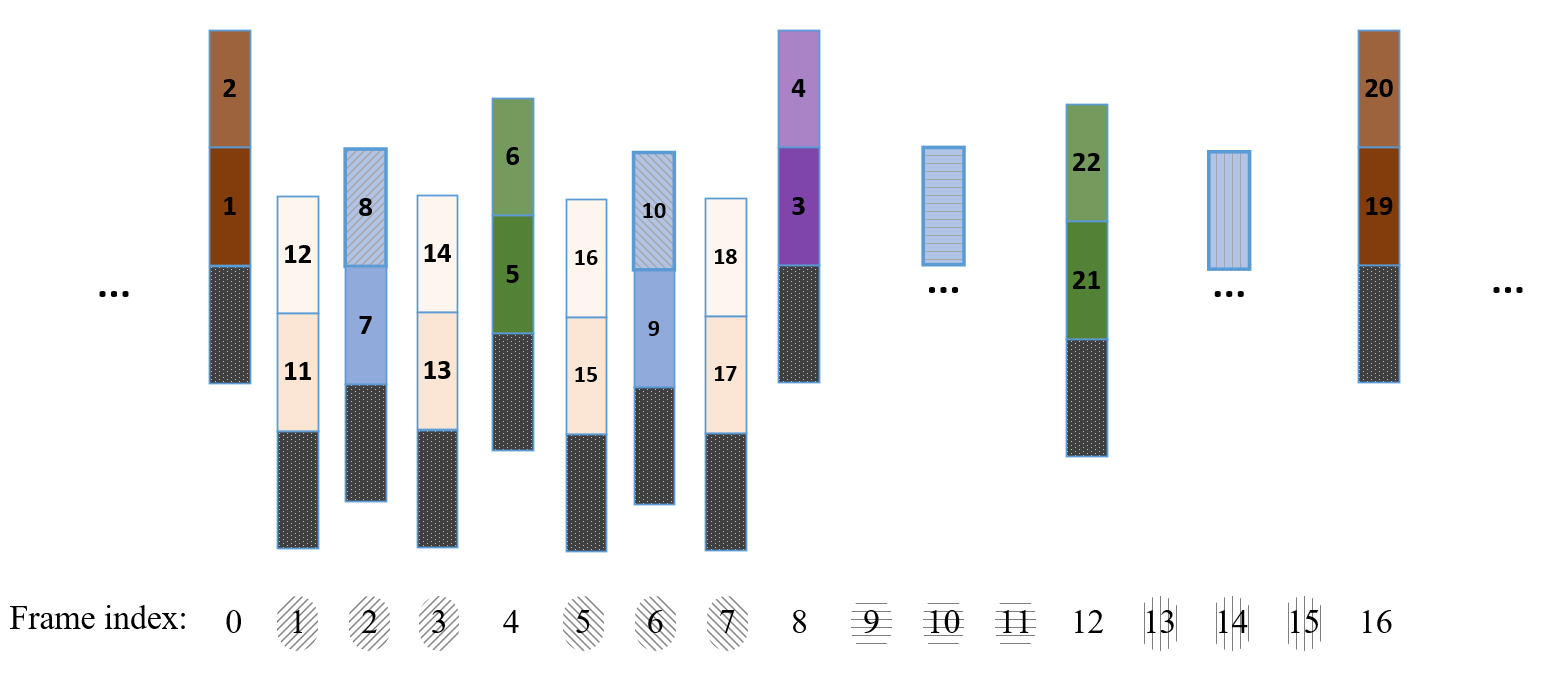
\includegraphics[width = 0.8\linewidth]{GOP-Structure.png}
\caption{Group of pictures (GOP) in SVC \label{fig:GOP_Structure}}
\end{figure}
 
Consider a video bitstream with 8-frame GOPs, as shown in Fig. \ref{fig:GOP_Structure}. Base layer packets are colored black, and enhancement packets with the same color are allocated into one group. In each group, error vectors of the enhancement packets can be calculated simultaneously, since the pixel errors they can cause do not interfere with each other. For example, the removal of packet 8 would cause pixel errors only in frame 1, 2 and 3, while packet 10 only in frame 5, 6 and 7 (frame index starts from 0). Therefore, we can perform only one subtraction for this group, to obtain error vectors $e_{8}$ and $e_{10}$, for both packets 8 and 10, as well as peer packets in all other GOPs. Note that these error vectors are highly sparse ones, because the discarding of a single enhancement packet can bring distortion only to a limited number of frames. To acquire all error vectors, the number of required extraction and decoding is approximately the number of enhancement layers $(L_Q - 1)$ times the number of temporal layers $L_T$. For the example in Fig. \ref{fig:GOP_Structure}, $L_Q = 3$ and $L_T = 4$, thus the extraction-and-decoding number would be $(3 - 1) \times 4 = 8$. However, we have to perform the same manipulation for $L_Q - 1 = 2$ more times, to dissociate the distortion impact of ``key frame'' \cite{H264Overview} (e.g. frame 0, 8, 16) packets. The loss of one enhancement packet in a key frame would bring distortion to two neighboring GOPs. As an instance, the loss of packet 4 would propagate error into frame 1 to frame 15, which would interfere with the distortion impact of packets in frame 0 (packet 1, 2) and 16 (packet 19, 20). Therefore, key frame enhancement packets within the same quality layer (e.g. packet 2, 4 and 20) should be allocated in two groups -- one for key frame packets of even-numbered GOPs (packet 2 and 20), the other for those of odd-numbered GOPs (packet 4). The actual extraction-and-decoding number for error vector acquisition is $(L_Q - 1) \cdot (L_T + 1)$, approximately the same as that for the Quality Layer information acquisition in JSVM \cite{Amonou07}.
 
\subsection{Distortion Estimation and Model Verification}
\label{subsec:distortion-estimation}

Based on the LEM, we can estimate the distortion caused by discarding any set of enhancement packets, by adding up the error vector of each packet in that set.

For example, consider a video sequence decoded from a sub-stream which is extracted by discarding packet set $I_x$. The error between this sequence and the original sequence can be estimated as
\begin{equation}
\label{eq:subset_error}
e(I_x) = e_{full} + \sum_{i \in {I_x}} e_i \: .
\end{equation}
Eq. (\ref{eq:subset_error}) has taken into consideration the error between the video sequence decoded from full enhancement packets and the original sequence, written as $e_{full}$.

Before using the estimation based on LEM, we conduct an experiment to verify its accuracy. Bitstreams in the experiment are encoded using the JSVM encoder, with the GOP structure illustrated in Fig. \ref{fig:GOP_Structure} and the CABAC entropy coding. Each bitstream contains one base layer and one enhancement layer, with QP = 33 and QP = 27, respectively. The enhancement layer is further divided into 2 Medium Grain Scalability (MGS) layers by configuring the MGS vector to separate the transform coefficients into two groups (containing 4 and 12 coefficients respectively). Random combinations of enhancement packets are removed from a bitstream, and the distortion estimated by the linear error model is compared with the distortion actually calculated after real decoding. Decoding is performed by the JSVM decoder, while other operations are performed with MATLAB. One comparison result for the test sequence {\em Foreman} (only the first 33 frames are used) is shown in Fig. \ref{fig:model_verification}. The horizontal axis denotes the frame index, and the vertical axis denotes the MSE measurement. The solid line represents the actual distortion of the frames, and the dotted line represents the distortion estimated by the proposed linear error model. It can be seen that the two lines are very close to each other, which demonstrates the accuracy of estimation using the proposed model. Estimation errors for all the eight SVC standard test sequences are listed in Table \ref{tab:estimation-error}, which shows that the average error is only about 5\%.

\begin{figure}[t]
\centering
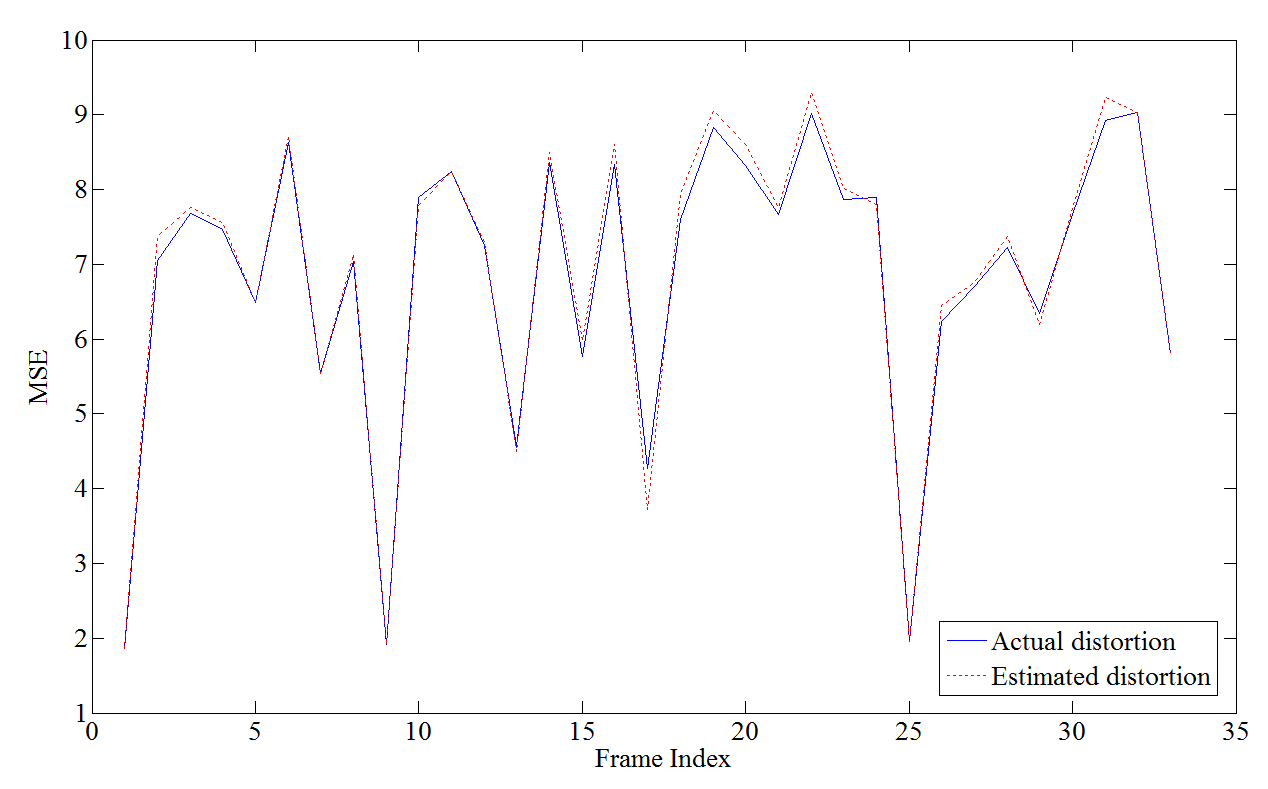
\includegraphics[width = 0.8\linewidth]{ModelVerification.png}
\caption{Comparison of the actual and the estimated distortion for sequence {\em Foreman} \label{fig:model_verification}}
\end{figure}

\begin{table*}
\centering
\caption{Performance of distortion estimation using LEM}
\label{tab:estimation-error}
\begin{tabular}{c|*{8}{p{1.2cm}<{\centering}|}{p{1.2cm}<{\centering}}}
	\hline\hline
	Sequence name & {\em Bus} & {\em City} & {\em Crew} & {\em Football} & {\em Foreman} & {\em Harbour} & {\em Mobile} & {\em Soccer} & \textbf{Average} \\ \hline
	Estimation error  & 2.83\% & 2.39\% & 10.36\% & 7.08\% & 4.95\% & 2.63\% & 5.77\% & 5.26\% & \textbf{5.16\%} \\ \hline
\end{tabular}
\end{table*}

\subsection{Priority Assignment and Bitstream Extraction}
\label{subsec:priority-assign}

In this subsection, we utilize the linear error model to enable R-D optimized bitstream extraction. Because finding the global optimal solution of the bitstream extraction problem is impractical, our bitstream extraction method uses a greedy algorithm \cite{GreedyAlgo} to obtain a sub-optimal solution. Note that the greedy algorithm is able to find a local optimum. However, the gap between the local optimum and the global optimum is uncertain. Similar to the greedy solution of the ``0-1 Knapsack Problem", every time a packet is to be discarded, we choose the packet that has the minimal R-D impact. A packet's R-D impact is mathematically measured by:
\begin{equation}
\label{eq:rd_impact}
\Phi = \dfrac{\partial D}{\partial R} \: ,
\end{equation}
where $\partial D$ represents the distortion change brought by discarding this packet, and $\partial R$ is the corresponding rate change. $\partial R$ is simply equivalent to the size of this packet, while $\partial D$ needs to be calculated by subtracting the distortions before and after the packet is discarded.

We simulate the process of discarding all the enhancement packets from a stream, using the above greedy strategy. During this process, the discarding order of a packet is regarded as its priority and recorded. Then, the packet priority values can be stored in the bitstream (either in the priority identifier field of the NALU header or in supplementary enhancement information messages) for real extraction in the future.

For long video sequences, an optimization window containing a certain number of frames is required, and the priority assignment and bitstream extraction are conducted independently in each window. Suppose the size of the optimization window, i.e., the number of frames involved in the above process, is $K$, and each frame contains $L_Q$ quality layers (one base layer and $L_Q-1$ enhancement layers). Then, the total number of enhancement packets to be discarded is $K \cdot (L_Q-1)$, and in every greedy step, there are at most $K$ packets, i.e., the packets currently at the top of every frame (see analysis in \ref{subsec:analysis-extraction}), that can be selected for discarding. Given that, the priority assignment process in each optimization window can be described in Algorithm \ref{algo:greedy}, with some terms in it explained below. The initial value $e_{full}$ is the error between the video sequence decoded from full enhancement packets and the original video sequence, as already introduced in (\ref{eq:subset_error}). $\Phi_m$ is defined as:
\begin{equation}
\label{eq:R-D_impact_m}
\Phi_m = \min_{i \in I_{top}} \Phi_i \: ,
\end{equation}
where $I_{top}$ stands for the top-layer packets, those currently able to be discarded, and $\Phi_i$ denotes the RD impact of packet $i$. $\Phi_i$ is calculated based on (\ref{eq:rd_impact}):
\begin{equation}
\label{eq:R-D_impact_i}
\Phi_i = \dfrac{\partial D}{\partial R} = \dfrac{PSNR(e_{seq}) - PSNR(e_{seq} + e_i)}{SIZE(i)} \:,
\end{equation}
where $SIZE(i)$ is the size of packet $i$, and $PSNR(*)$ is the function for obtaining PSNR from an error vector. For clarification, PSNR is defined using the mean squared error (MSE), i.e., the average of the squares of the elements in the error vector.

\begin{algorithm}
\caption{Greedy-like priority assignment algorithm}
\label{algo:greedy}
\begin{algorithmic}
    \STATE Initialize $e_{seq}$ to $e_{full}$, and initialize $q$ to 0.
    \WHILE{$q < K \cdot (L_Q - 1)$}
	    \FOR{the (at most) $K$ top layer packets}
		    \STATE Find the packet $m$ that has the least RD impact $\Phi_m$
		\ENDFOR
		\STATE Set the priority value of packet $m$ to $q$
		\STATE Remove $m$ from the sequence
		\STATE Update $e_{seq}$ to $e_{seq} + e_m$, and update $q$ to $q+1$
    \ENDWHILE
\end{algorithmic}
\end{algorithm}

It is easy to see that the computational complexity of this priority assignment algorithm is $O(K^2)$. Note that, the computation in this priority assignment process is actually very insignificant compared with the decoding process required for the error vector acquisition. With a larger optimization window size $K$, we would have more packets to compare and determine their priorities each time, which will potentially result in more optimized extraction. However, doing this will also require more computation and, more noticeably, increase the memory used to store the error vectors. Besides, if the priority values are to be stored and signaled using the 6-bit priority identifier field of the NALU header \cite{Amonou07}, only a range of 0$\sim$63 is supported, which also limits the value of $K$.

\subsection{The No-Reference Case}
\label{subsec:noref-case}

In some scenarios, the priority assignment and bitstream extraction need to be conducted without access to the original video sequence. This would make the bitstream extraction a more difficult problem, because the distortion is harder to obtain as the reference signal is not available. This ``no-reference bitstream extraction'' problem is actually more frequently encountered in real practice, because it is more common for the streaming service provider to have a compressed bitstream rather than the video source. In this subsection, we consider this no-reference case and modify the proposed algorithm to meet the special characteristics caused by lacking of reference.

Without the original video sequence, we cannot obtain the error between the video sequence decoded from full enhancement packets and the original sequence, which is $e_{full}$ used in \ref{algo:greedy}. A straightforward idea is setting $e_{full}$ to zero, which means that all distortions are calculated with respect to the fully reconstructed signal, rather than the original sequence. However, simply doing so causes the algorithm to perform badly in experiments. It is found that, as discarding some enhancement packets will not result in much significant error, the calculated PSNR values are too large to properly represent the real distortion. To address this issue, instead of calculating the PSNR, we directly use the MSE of all pixels as the distortion criteria in the priority assignment algorithm. This proves to be an effective solution, and the extraction performance turns out to be improved.

After each packet is assigned a priority value and an optimized extraction is made possible, the video stream can now adapt to different bitrates well. Next, we propose a quality control algorithm based on the PID mechanism, which is responsible for determining the suitable bitrate for transmission according to the current network conditions.

%%%%%%%%%%%%%%%%%%%%%%%%%%%%%%%%%%%%%%%%%%%%%%%%%%%%%%%%%%%%%
\section{PID-based Quality Control Algorithm}
\label{sec:quality-control}

The PID controller \cite{PID}\cite{Astrom02} is a control loop feedback mechanism commonly used in industrial control systems. \textit{Process variable} and \textit{setpoint} are two core concepts in PID control. The process variable stands for the current status of the system. The setpoint is the target for this system to reach. The goal of PID control is to minimize the error between the process variable and the setpoint. The controller output $u(t)$ is defined as follows:
\begin{equation}
\label{eq:pid-output}
u(t) = {K_p} \cdot e(t) + {K_i} \cdot \int_0^t {e(\tau )d\tau }  + {K_d} \cdot \frac{d}{{dt}}e(t) \: ,
\end{equation}
where $e(t)$ represents the error between the process variable and the setpoint at time $t$. $K_p$, $K_i$, and $K_d$ here are tuning parameters that represent the proportional gain, integral gain and derivative gain, respectively. The result of (\ref{eq:pid-output}) is used for manipulating the system to make the process variable change towards the setpoint.

As an effective and flexible control technique, PID control has been used to solve many kinds of control problems. In the area of video coding, we notice that PID is utilized to design rate control algorithms (rate control in video coding mainly involves adjusting the encoding parameters for every frame, so that the bits are appropriately allocated and the desired bitrate is achieved) \cite{Wong04}. We also notice that some researchers have proposed a theoretical model or middle-ware framework for QoS adaptation \cite{Li98} \cite{Li99}, with PID as the basic control scheme. However, we have not found any paper that integrates the PID method into the quality control of video streaming. While rate control of video coding and quality control of video streaming are two different problems, they do share some common properties, such as the buffer mechanism and the requirement for smoothness. We are therefore inspired to design a PID-based quality control algorithm and utilize it to deliver better video quality to the user.

In this section, we first introduce the \textit{quality level} concept to discretize the bitrate and quality of a scalable video. Then we define the process variable used in our PID-based quality control algorithm. After that, the algorithm is formulated and explained in detail, followed by a brief discussion on parameter selection.

\subsection{Quality Level}
\label{subsec:quality-level}

The video quality is a continuous value, and it is impractical to control it at an arbitrary precision. Therefore, we propose a \textit{quality level} concept for a discrete description of the video quality. When the video quality is to be adjusted, we simply increase or decrease the quality level. Each quality level corresponds to a certain bitrate. A higher quality level corresponds to a higher bitrate, and vice versa. The number of quality levels and how they are mapped to sub-streams with different bitrates depend on the actual requirements or implementation. The more quality levels are defined, the more precisely the control algorithm can adjust bitrate to follow the bandwidth change. As pointed out in section \ref{sec:intro}, simulcast streaming systems can only have limited quality levels while SVC streaming systems can define quality levels at a much finer granularity.

\subsection{Process Variable Selection}
\label{subsec:process-variable}

In our PID-based quality control algorithm, the process variable is called \textit{actual\_check interval ratio}, which is defined as follows.

In DSS, two timelines are important. Push timeline indicates the time of pushing video data packets to the streaming buffer, and play timeline indicates the time these data packet should be played, i.e., the presentation time stamp (often seen as PTS) of each packet. Their relationship is shown in Fig. \ref{fig:intervals}. The program will check the timelines periodically, and, in the default quality control algorithm of DSS, use the packet delays to decide whether quality change is needed. The two intervals shown in Fig. \ref{fig:intervals}, i.e., check interval and actual interval, are worth noticing and may provide useful information. In the ideal situation, during each check interval, the server pushes an amount of data that will actually play for a period of time equal to the check interval, i.e., \textit{actual\_interval} = \textit{check\_interval}. If \textit{actual\_interval} is smaller than \textit{check\_interval}, it means that less data is pushed to the client, and the pushing is slowed down because bandwidth is relatively low at this time. On the other hand, if \textit{actual\_interval} is larger than \textit{check\_interval}, it indicates that the network conditions are good and the data are being pushed quickly to the client. The ratio of these two intervals, i.e., \textit{actual\_check interval ratio}, is in direct proportion to the ratio of the bitrate suitable for the network conditions and the bitrate currently being used.

The \textit{actual\_check interval ratio} is suitable for use in quality control because: 1) this ratio directly reflects the mismatch of the current pushing bitrate and the bandwidth, and by adjusting the bitrate according to it, this ratio can be used to accurately change the video quality; 2) the desired value of this ratio is 1.0 by definition, therefore, we do not need to determine the optimized setpoint using mathematical methods or experiments; and 3) it is easy to compute and implement in practical systems.

\begin{figure}[t]
\centering
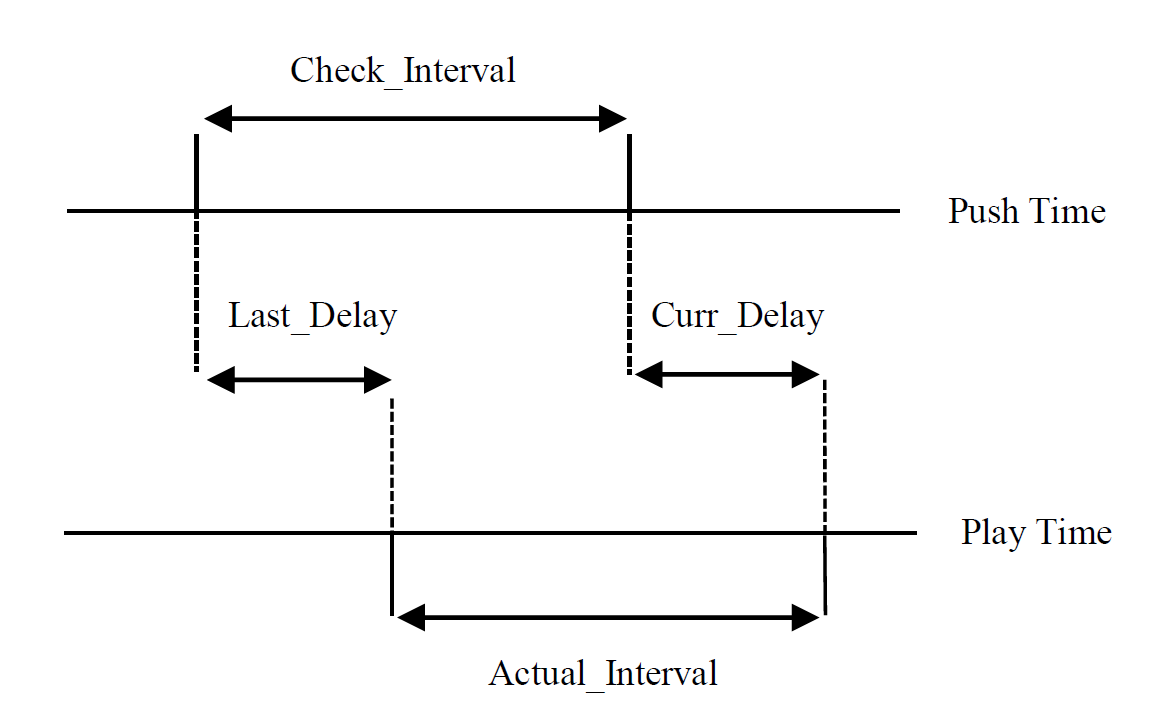
\includegraphics[width = 0.9\linewidth]{Intervals.png}
\caption{Two timelines in the Darwin Streaming Sever (DSS) \label{fig:intervals}}
\end{figure}

\subsection{Model Formulation}
\label{subsec:model-formulation}

In normal PID control, the controller output is calculated using the proportion, integral and differential of the error between the process variable and the setpoint, as shown in (\ref{eq:pid-output}). Considering that the chosen process variable is a ratio and the corresponding setpoint is 1, we make a little modification to the general PID controller and obtain a ratio-based model. In this model, the ratio is directly used to calculate the controller output, and all subtraction operations in the original PID equations have been properly changed to division operations for correctness, as follows:

\begin{equation}
\label{eq:ut}
{u_t} = {K_p} \cdot E_p^t + {K_i} \cdot E_i^t + {K_d} \cdot E_d^t ,
\end{equation}

\begin{equation}
\label{eq:ep}
E_p^t = \frac{{actual\_interva{l_t}}}{{check\_interva{l_t}}} ,
\end{equation}

\begin{equation}
\label{eq:ei}
E_i^t = \frac{{long\_actual\_interva{l_t}}}{{long\_check\_interva{l_t}}} ,
\end{equation}

\begin{equation}
\label{eq:ed}
E_d^t = E_p^t/E_p^{t - 1} ,
\end{equation}

\begin{equation}
\label{eq:long-actual}
long\_actual\_interva{l_t} = \sum\limits_{\tau = {T_l}}^t {actual\_interva{l_\tau}} ,
\end{equation}

\begin{equation}
\label{eq:long-check}
long\_check\_interva{l_t} = \sum\limits_{\tau = {T_l}}^t {check\_interva{l_\tau}} .
\end{equation}


In (\ref{eq:ut}), $K_p$, $K_i$, and $K_d$ indicate the tuning parameter for the proportional, integral and derivative part, respectively, and $E_p^t$, $E_i^t$, $E_d^t$ stand for the corresponding observed values for each part, which are defined in (\ref{eq:ep})-(\ref{eq:long-check}); the controller output $u_t$ is utilized to calculate a suitable bitrate for transmission and further to determine which quality level should be selected (see Algorithm \ref{algo:control} for more details).

In (\ref{eq:long-actual}) and (\ref{eq:long-check}), $T_l$ stands for the last quality change time. Theoretically, the integral part should be recorded and calculated since the system starts. In practice, however, the bandwidth may change significantly during the transmission. If the integral part is recorded for too long time, it may fail to reflect the current network conditions and thus slow down the reaction for better quality levels. A compromise here is to choose a relatively long time, i.e., the time from last quality change till now, for the calculation of the integral part.

This ratio-based model is more simple and effective for the chosen process variable and setpoint. Moreover, in this model, the controller output has intuitive meaning when the three parameters are normalized. It is easy to see that $E_p^t$, $E_i^t$, $E_d^t$ are all ratios with a value around 1, and the controller output $u_t$ can be seen as a weighted average of the three ratios, with the three parameters as weights. Therefore, the controller output is also a ratio with a value around 1, which reflects the relationship between the bitrate suitable for the network conditions and the bitrate currently being used. In other words, if the output is larger than 1, then the controller has determined that the bitrate should be increased accordingly, and vice versa. Use it as a multiplier to manipulate the bitrate currently being used, and we would be able to control the streaming system to match the network conditions.

The proposed algorithm is described in Algorithm \ref{algo:control}. Compared to other scheduling strategies, this quality control algorithm has several advantages. First, this algorithm does not just rely on the current packet delay or the information at a fixed time point; therefore, a quality change may occur at any proper time. Second, because the model takes prediction into account, it is able to decide whether the bandwidth will be high or low enough for the quality level to change in the near future, so as to avoid unnecessary quality changes. Third, in this algorithm it's not obliged to change one quality level at a time. This enables a fast quality drop to avoid latent playback pause when bandwidth suddenly decreases, as well as a fast quality rise to provide better video as soon as possible when system starts, resulting in a seamless watching experience, where the user can enjoy the video without stopping or waiting.

\begin{algorithm}
\caption{PID-based quality control algorithm}
\label{algo:control}
\begin{algorithmic}
    \STATE before packet is sent
    \STATE check\_interval = curr\_time -- last\_check\_time
    \STATE actual\_interval = curr\_media\_time -- last\_check\_media\_time
    \STATE long\_check\_interval += check\_interval
    \STATE long\_actual\_interval += actual\_interval
    \STATE calculate $E_p^t$, $E_i^t$, $E_d^t$ according to Eq. (\ref{eq:ep}) - (\ref{eq:ed})
    \STATE output = ${K_p} \cdot E_p^t + {K_i} \cdot E_i^t + {K_d} \cdot E_d^t$
    \STATE new\_bitrate = output * curr\_bitrate
    \STATE new\_level = get\_level(new\_bitrate, bitrate\_of\_level[])
    \IF {quality level changed}
    	\STATE long\_check\_interval = 0
    	\STATE long\_actual\_interval = 0
    	\STATE curr\_bitrate = bitrate\_of\_level[new\_level]
    \ENDIF
    \STATE send packet according to the new quality level
\end{algorithmic}
\end{algorithm}


\subsection{Parameter Selection}
\label{subsec:parameter-selection}

As with other PID control systems in the industry, the selection of the three parameters is implementation-dependent, and most of the time, manual tuning with trial and error is required to achieve optimal results. Each parameter has impacts on different aspects of the system, and knowing these impacts is useful for parameter selection. Generally, the proportional part in the PID controller affects the system's stability. If the proportional gain $K_p$ is too high, the system can become unstable. However, a low $K_p$ would result in a long rising time that makes the system response slow. In addition to eliminating the steady-state error, the integral term also accelerates the movement of the process value towards the setpoint, which means that increasing $K_i$ can reduce the rising time. However, because the integral part accumulates errors from the past, it can cause the present value to overshoot the setpoint value, and a too high $K_i$ will lead to instability as well. These can all be compensated by the derivative part, which predicts the system behavior and has the effect of reducing the overshoot, increasing the stability, and improving the settling time (the time taken to reach setpoint after a disturbance). The issue with the derivative part is that it is very sensitive to noise; therefore, industrial practices indicate that the derivative gain $K_d$ should usually stay low.

For the proposed quality control algorithm, the Ziegler--Nichols method \cite{Ziegler42} is used to select the parameters for better performance. This method is performed by setting the integral and derivative parameters to zero and then tuning $K_p$ to the value $K_u$ until the output begins to oscillate with constant amplitude. Assuming that the oscillation period is $T_u$, we set $K_p = 0.6K_u$, $K_i = 2K_u/T_u$, and $K_d = K_u \cdot T_u/8$. $K_p$, $K_i$, and $K_d$ are then normalized to obtain the final parameters. In the following experiments, the parameters are chosen as $K_p = 0.22$, $K_i = 0.73$, $K_d = 0.05$ using this method. With these parameters, the PID-controlled streaming system is stable, and also quickly begins to follow the bandwidth change, as shown by the experimental results in the next section.

We choose to use the standard Ziegler--Nichols method because it already considers each parameter's impacts and produces acceptably good results. Adopting more sophisticated or automated techniques to further optimize the parameter selection and controller performance will be our future work. The robustness of the controller can also be improved by adding a mechanism that dynamically adjusts the controller parameters based on environment and performance change. Note that in the video quality control algorithm, only the bitrate and the bandwidth are relevant, not the video content. Therefore, once the parameters are chosen, they should apply well to different video streams.


%%%%%%%%%%%%%%%%%%%%%%%%%%%%%%%%%%%%%%%%%%%%%%%%%%%%%%%%%%%%%
\section{Experimental Results}
\label{sec:experiment}

Implementing our proposed adaptive streaming system requires the combination of the optimized bitstream extraction and the PID-based quality control algorithm. The latter determines the current bitrate to follow the bandwidth change, and the former will ensure that the sub-stream with the best possible quality is obtained and sent under that bitrate constraint. They work together to improve the user's experience of watching online videos. With DSS as the implementation basis, we have integrated the proposed algorithms into it for the purpose of both research and applications.

In this section, we first present separate experiments to show the advantage of each proposed solution, and then present the result when they are combined together.

\subsection{Experiments for Bitstream Extraction}
\label{subsec:exp-extraction}

We compare the performance of the proposed bitstream extraction method with that of JSVM 9.16.

All the test bitstreams are encoded the same way as in the verification experiment of Section III-C. For each test bitstream, ten bitrate points (one with all enhancement packets, one with only the base layer packets, and 8 uniformly spaced points in between) are chosen for extraction. For each bitrate point, the extraction is conducted using the bitstream extractors in JSVM, with and without \textit{Quality Layers} (denoted as JSVM QL and JSVM Basic, respectively), and the proposed method. The size of the optimization window in the priority assignment process is 32 frames, i.e., 4 GOPs with a GOP size of 8. All of the eight SVC standard sequences with CIF resolution are considered at 30FPS and tested in our experiments.

The performance comparisons for City, Foreman, Harbour, and Soccer are shown in Fig. \ref{fig:extraction-performance}. It can be seen that the R-D curves of the proposed method are always on the top (with only one exception in Foreman). For each sequence, the maximum and average PSNR gain through all 10 bitrate points are calculated and listed in Table \ref{tab:extraction-gain}, which shows that our extraction method can achieve a significant performance gain compared with JSVM Basic, and also performs better than JSVM QL. Table \ref{tab:extraction-gain} also presents the results obtained when the optimization window size is set to 48 frames, i.e., 6 GOPs. It is demonstrated that a larger window size can increase the performance to some degree. However, it should be noted that, in our implementation of the proposed system, the optimization window is not that large, for the reason stated at the end of Section \ref{subsec:priority-assign}.

Regarding other bitstream extraction methods in addition to JSVM, the work in \cite{Maani09} achieves a much better performance than JSVM QL, and even better than ours. However, the method of \cite{Maani09} requires more computation in order to train robust model parameters for different sequences, while the complexity of our method is always the same with JSVM QL. As far as we know, without significantly increasing the complexity, it is difficult to achieve a large PSNR gain.

\begin{figure*}[t]
\centering
\subfloat[City]{
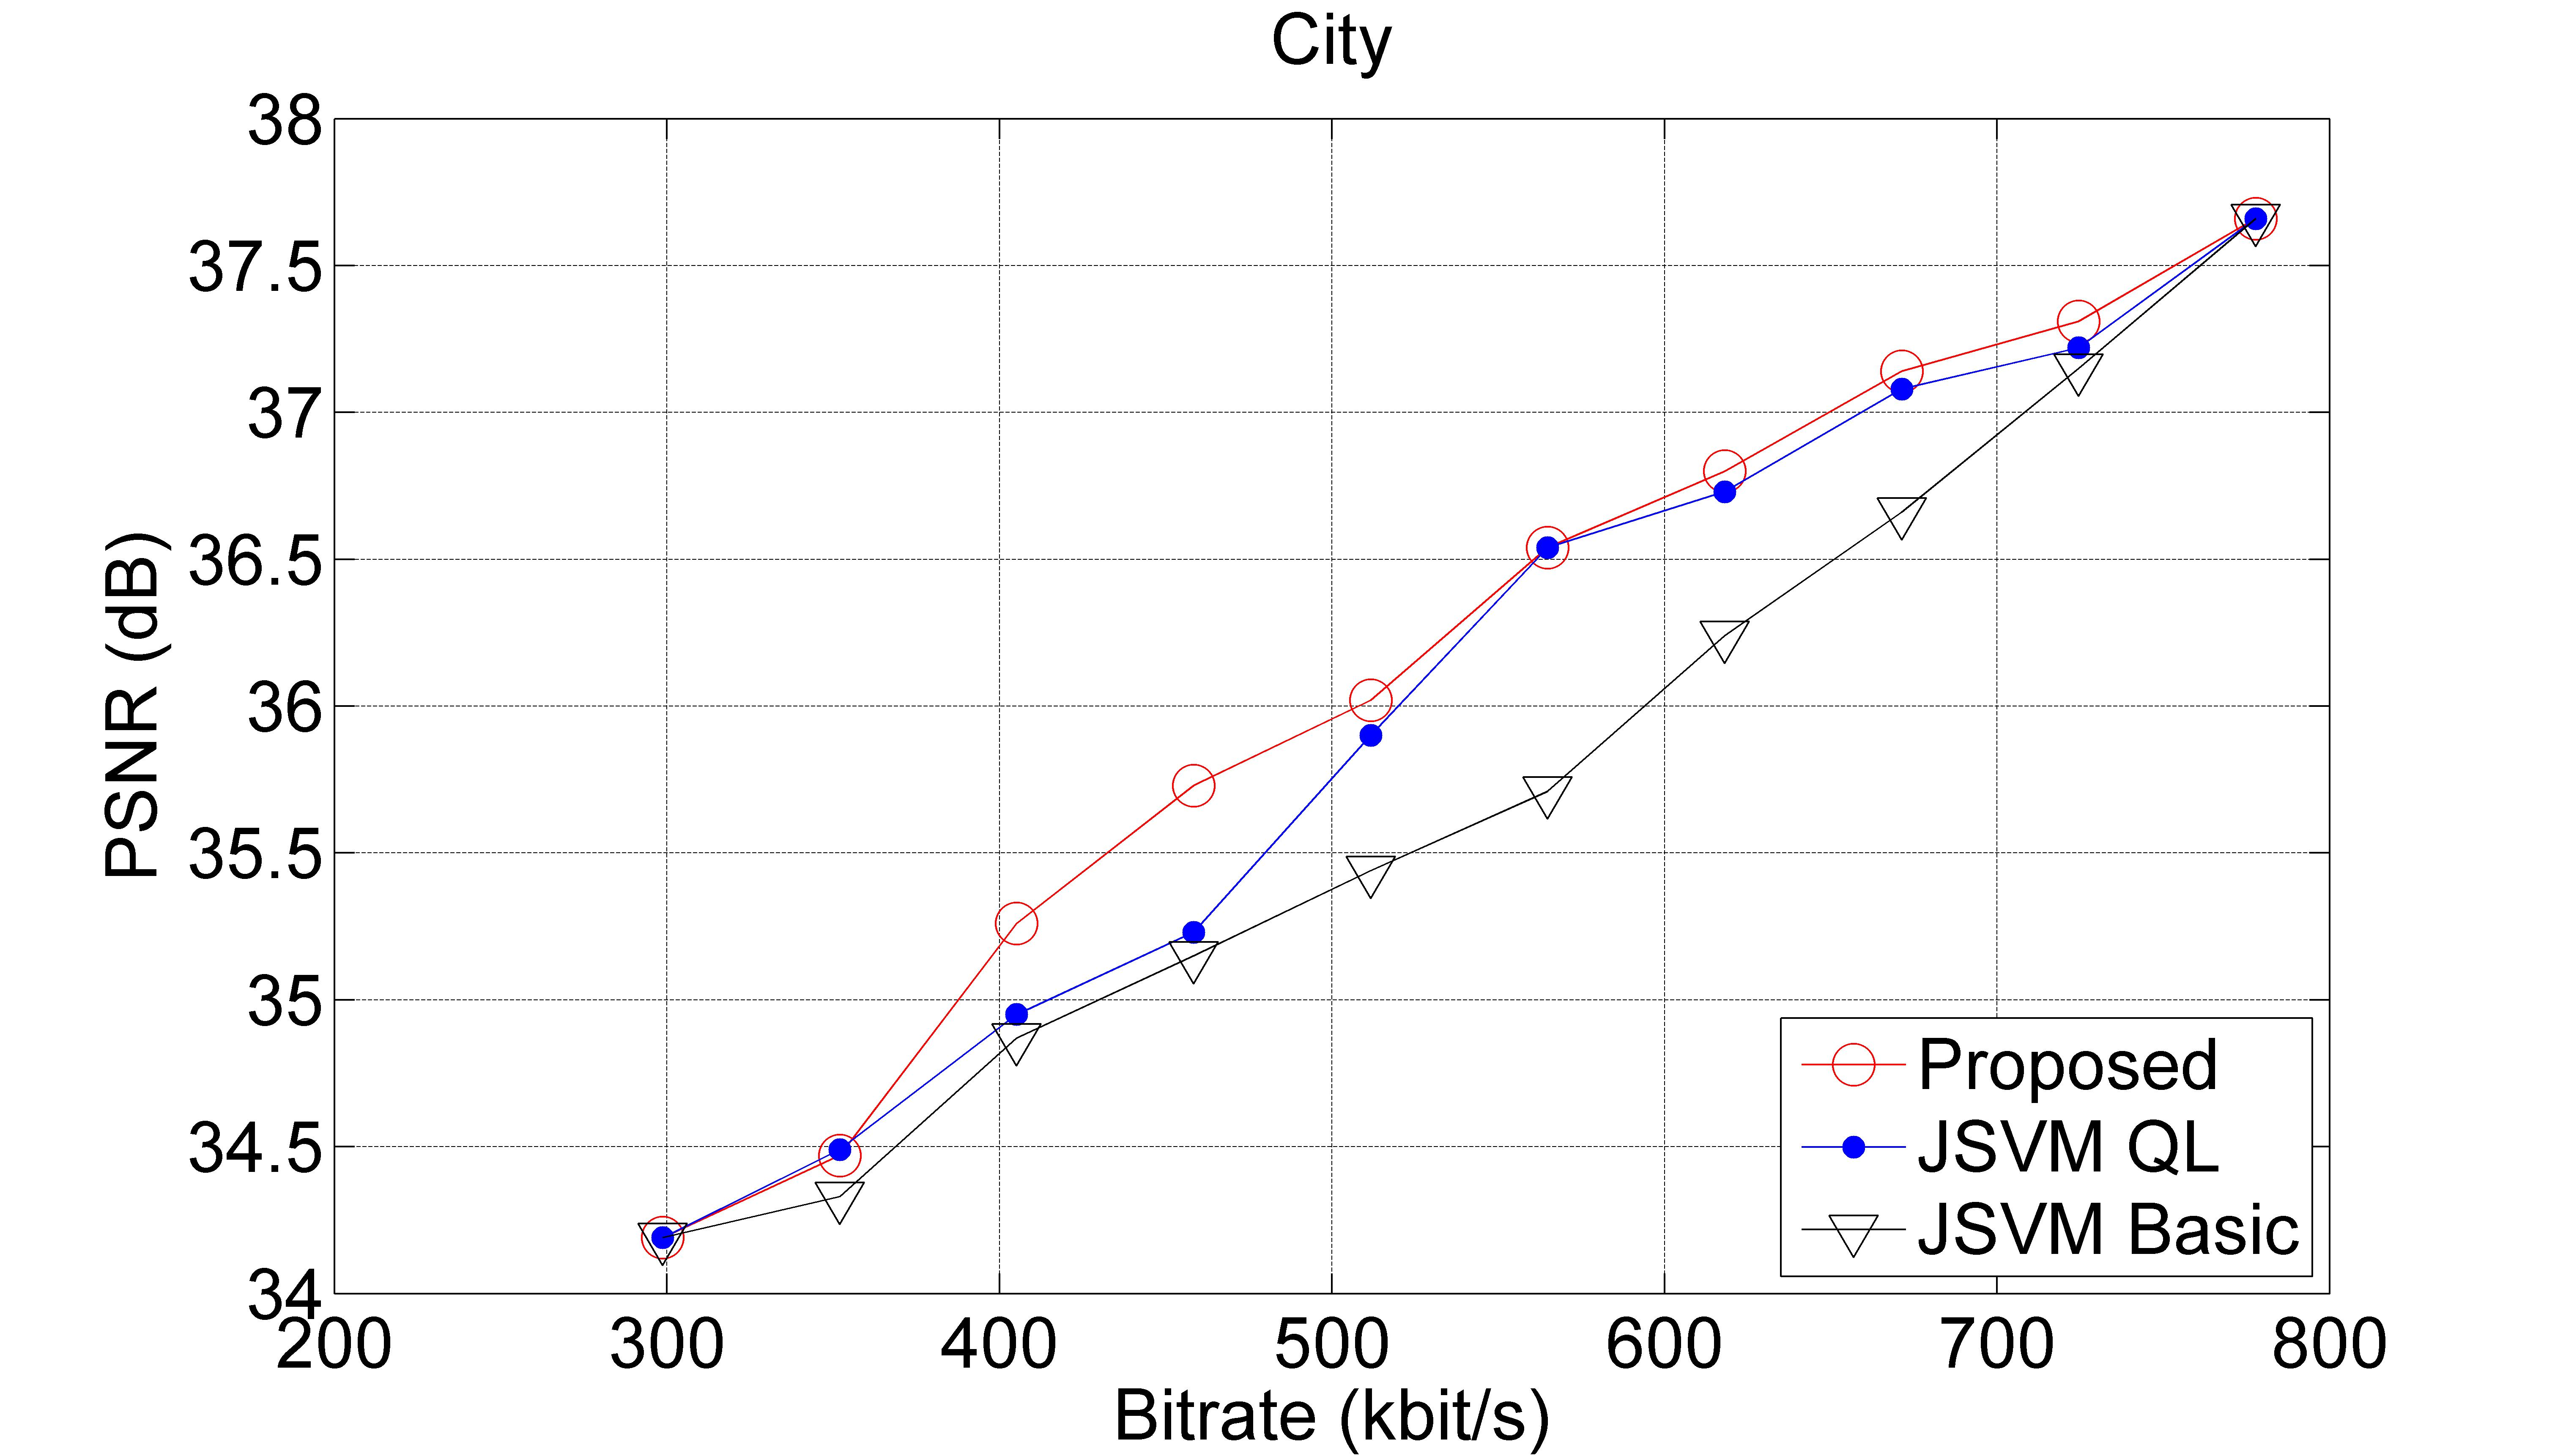
\includegraphics[width=0.40\textwidth]{City.jpg}
\label{fig:City}}
\subfloat[Foreman]{
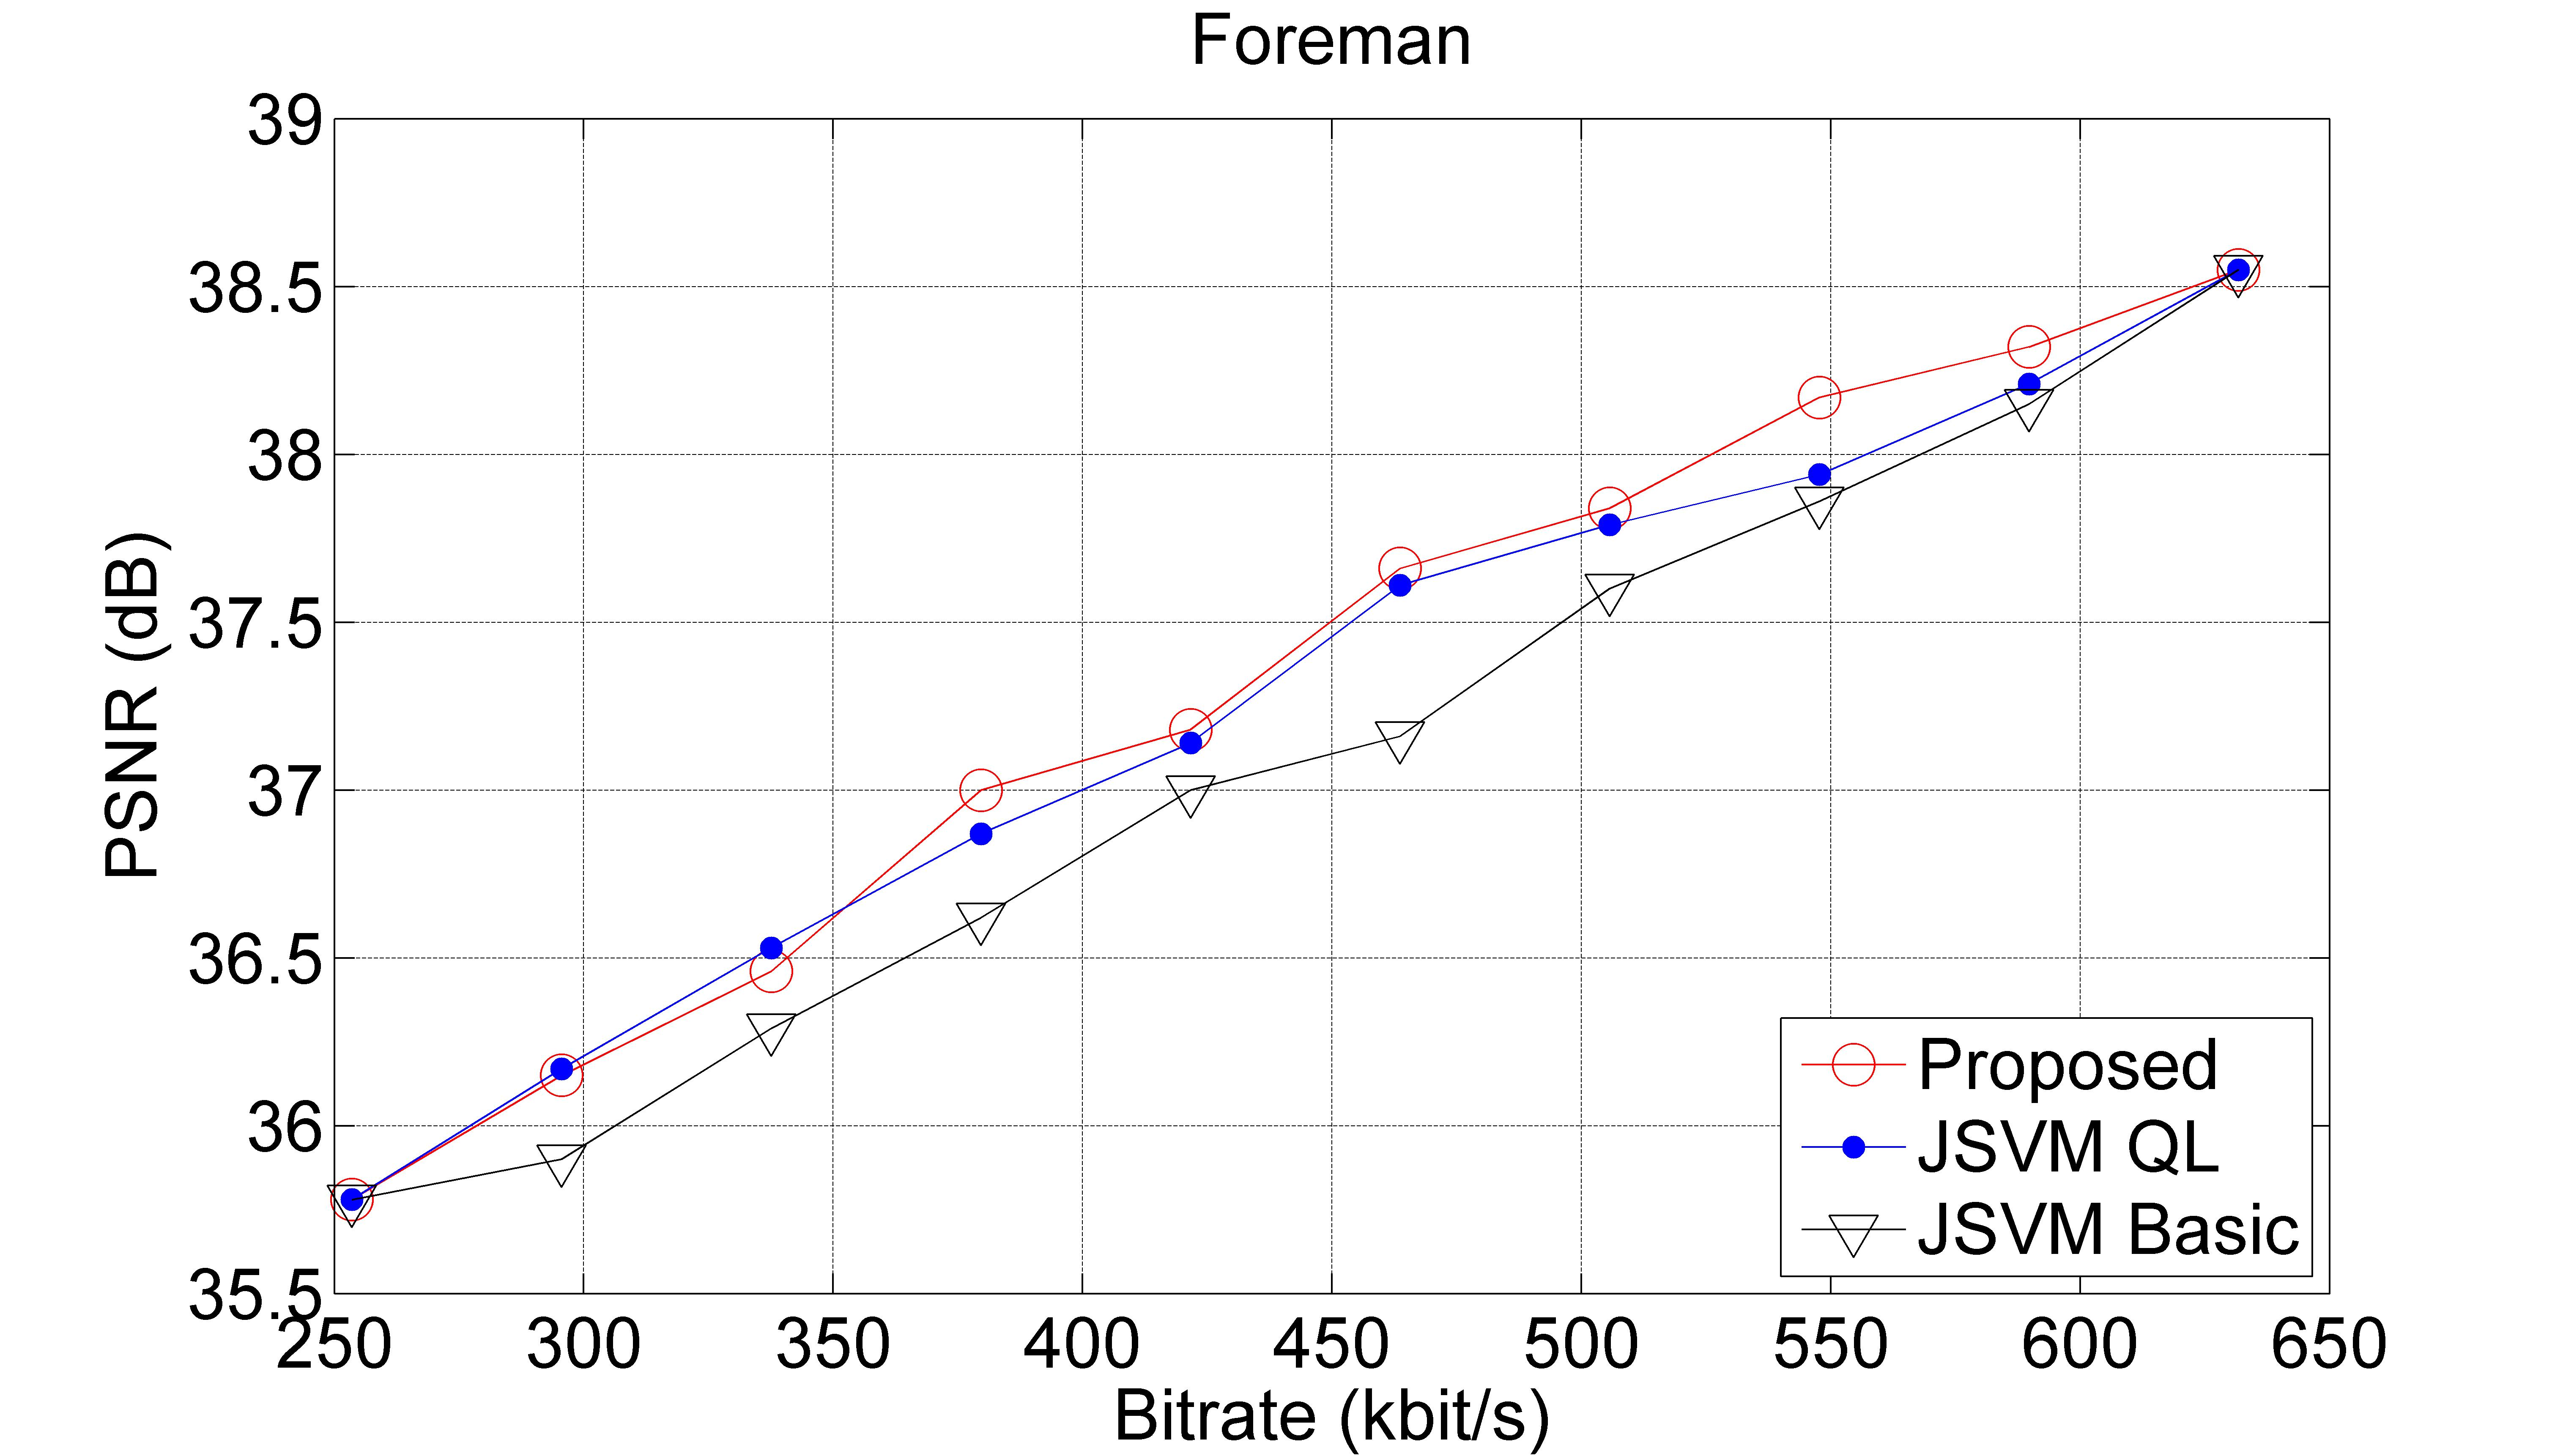
\includegraphics[width=0.40\textwidth]{Foreman.jpg}
\label{fig:Foreman}}
\qquad
\subfloat[Harbour]{
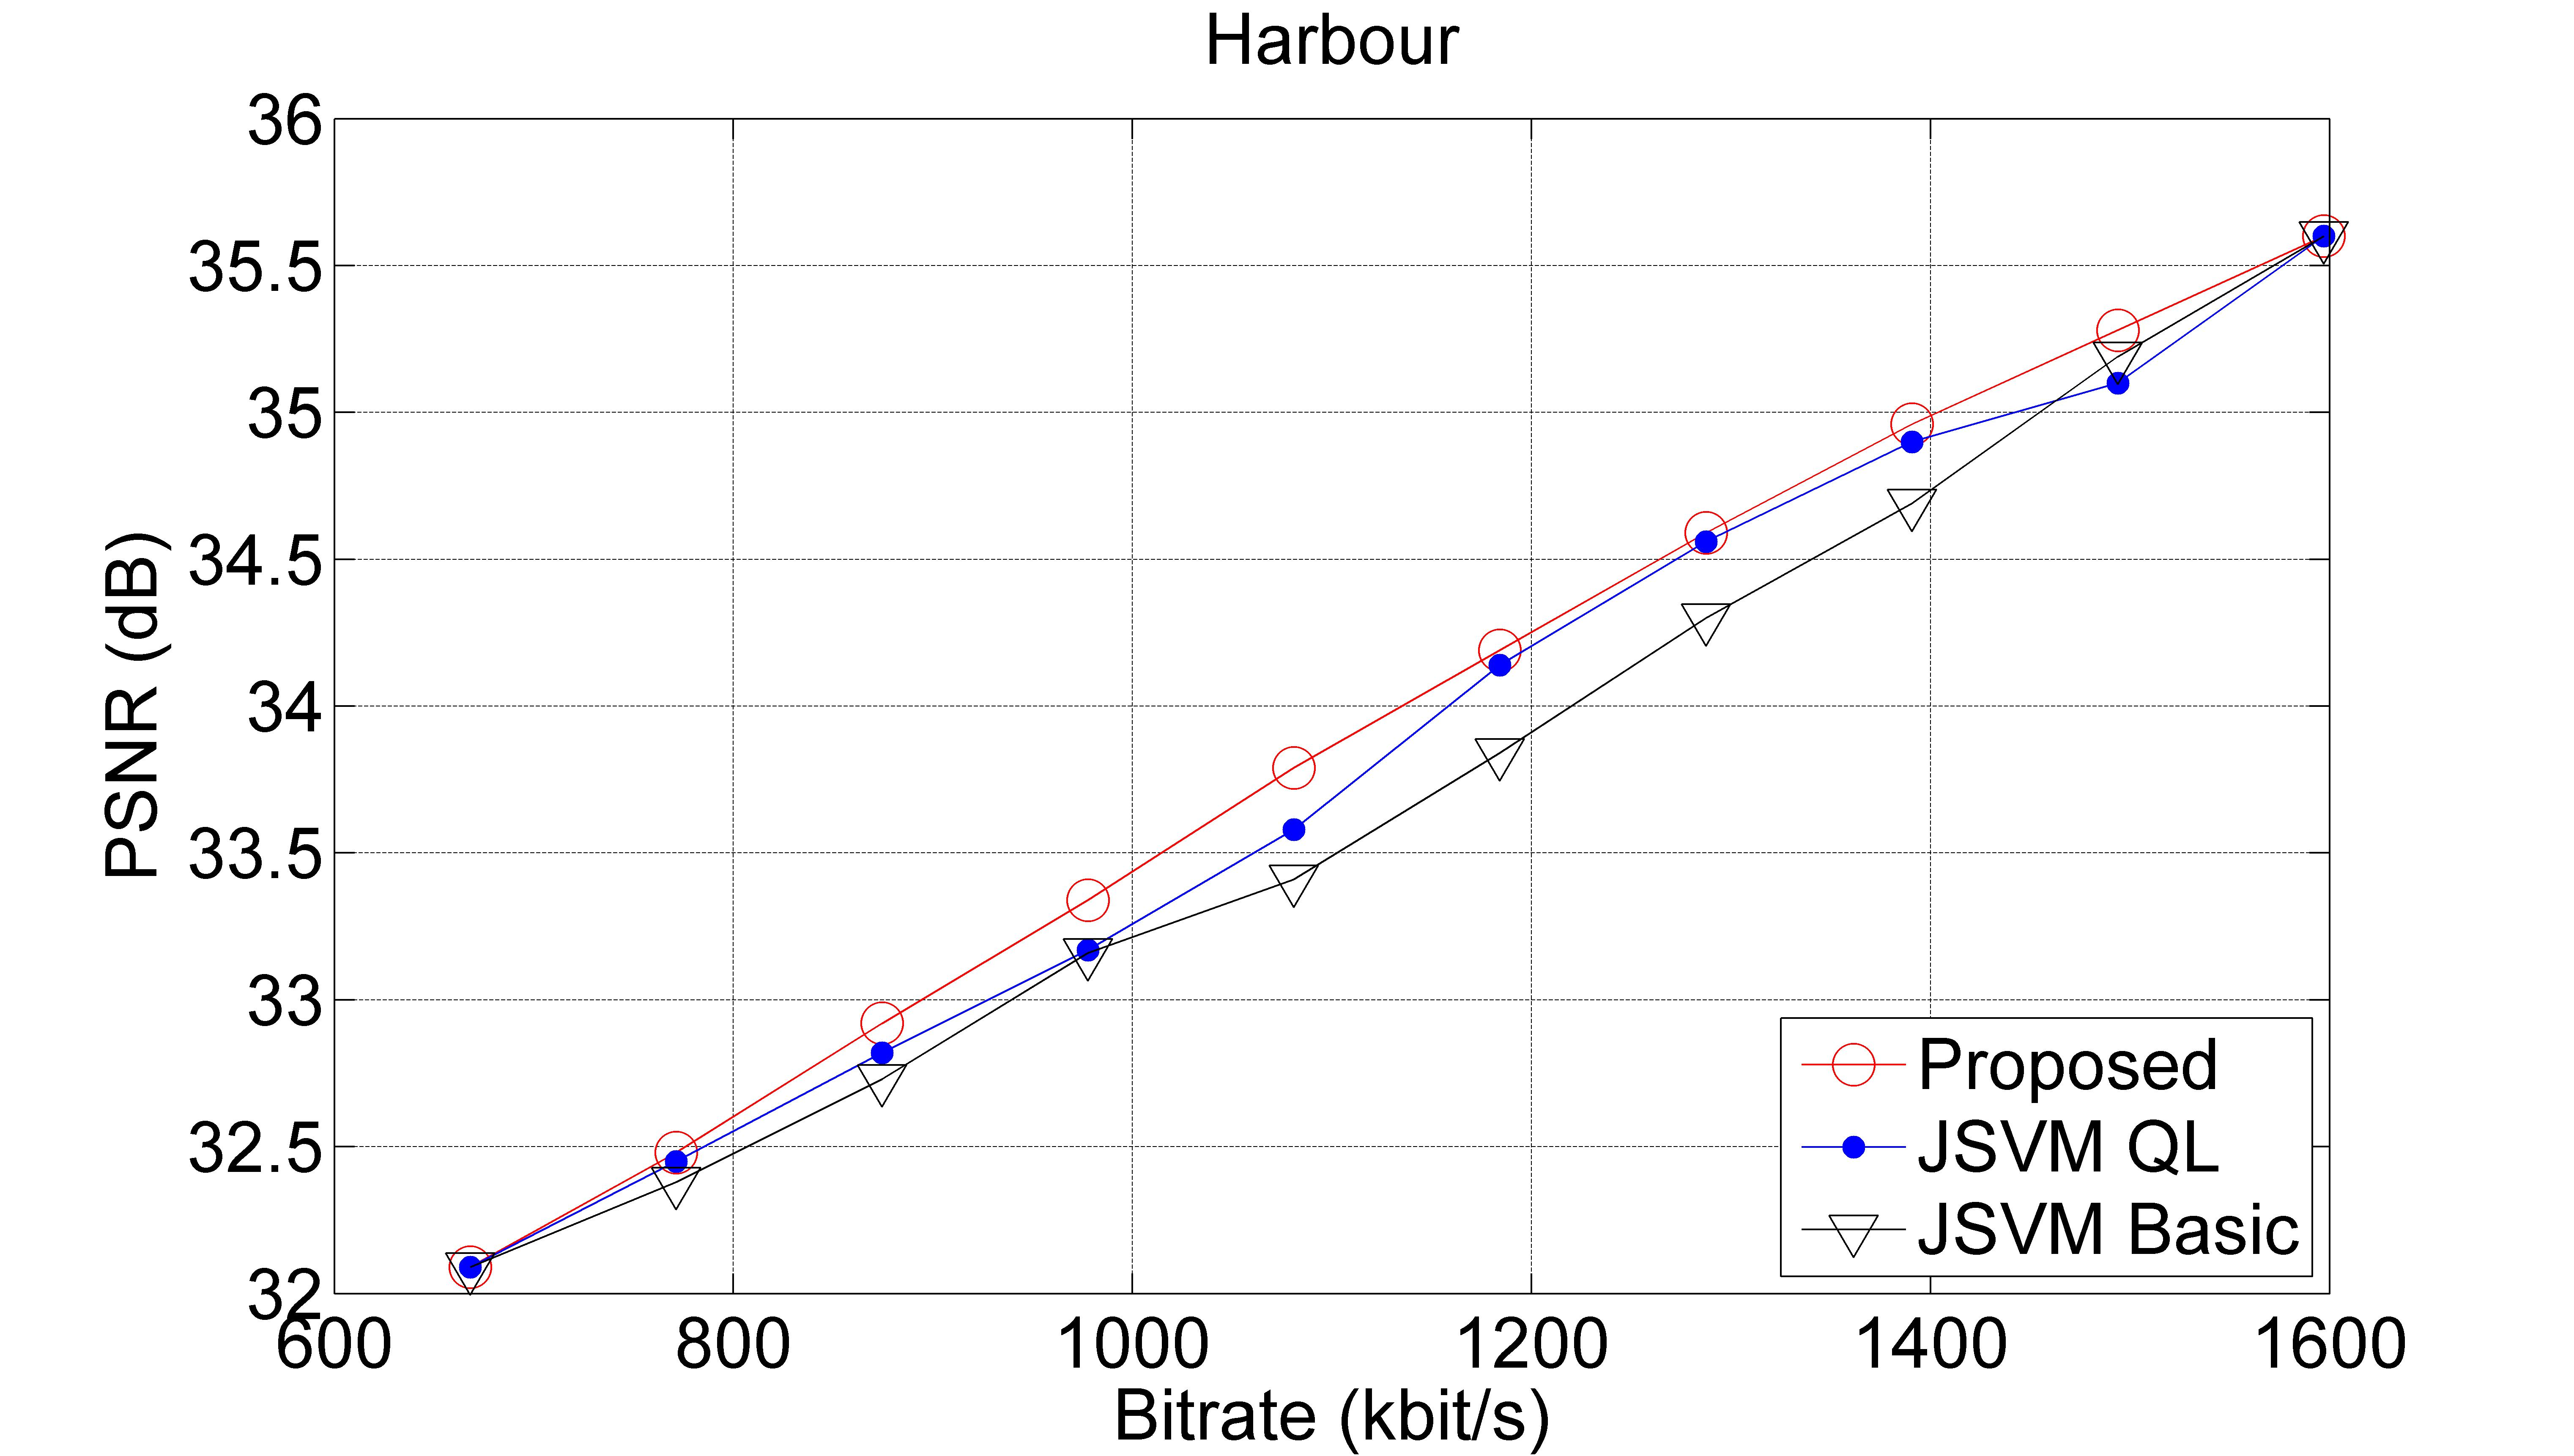
\includegraphics[width=0.40\textwidth]{Harbour.jpg}
\label{fig:Harbour}}
\subfloat[Soccer]{
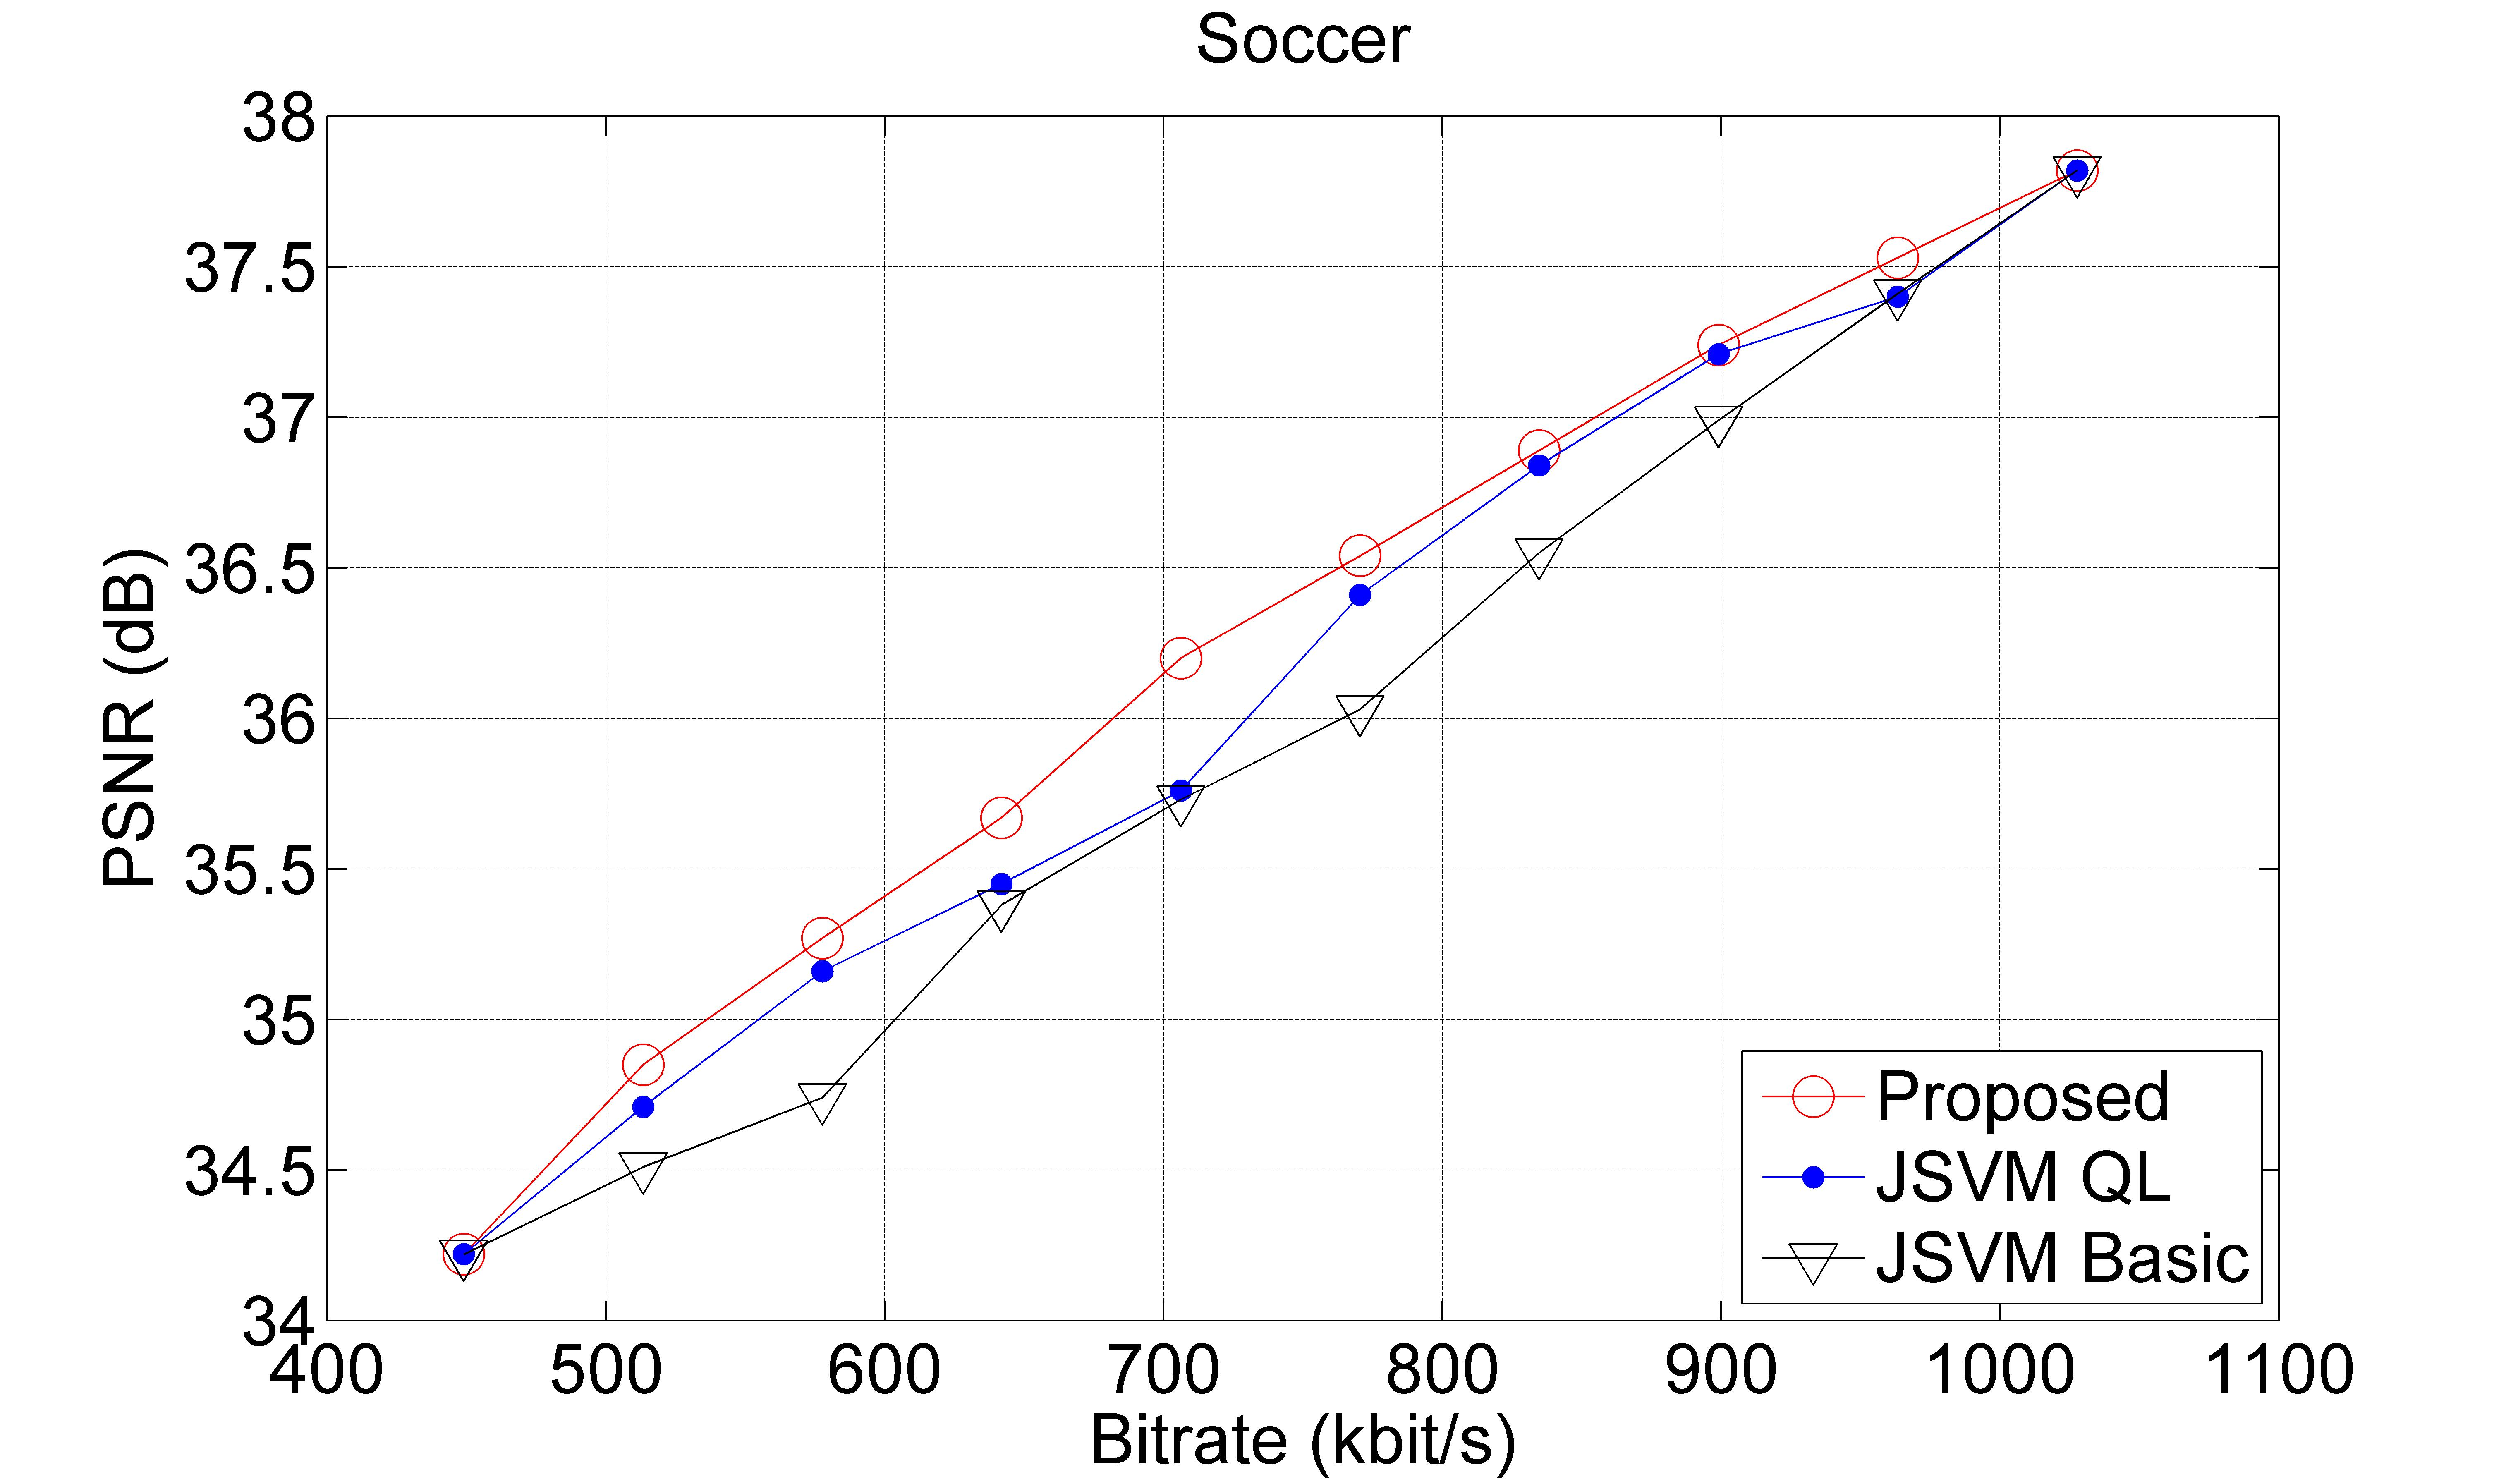
\includegraphics[width=0.40\textwidth]{Soccer.jpg}
\label{fig:Soccer}}
\caption{Performance of three bitstream extraction methods for various CIF sequences}
\label{fig:extraction-performance}
\end{figure*}

\begin{table*}[t]
\centering
\caption{Luma PSNR gain of the proposed algorithm compared with JSVM}
\label{tab:extraction-gain}
\begin{minipage}{0.95\linewidth}
% \renewcommand{\thefootnote}{\thempfootnote}
\centering
\begin{tabular}{c|c|p{1.2cm}<{\centering}|p{1.2cm}<{\centering}|p{1.2cm}<{\centering}|p{1.2cm}<{\centering}| 
p{1.2cm}<{\centering}|p{1.2cm}<{\centering}|p{1.2cm}<{\centering}|p{1.2cm}<{\centering}}
%% |l|l| to left justify each column entry
%% |c|c| to center each column entry
%% use of \rule[]{}{} below opens up each row
\hline \hline
\multicolumn{2}{c|}{Sequence} &
{\em Bus} & {\em City} & {\em Crew} & {\em Football} & {\em Foreman} & {\em Harbour} & {\em Mobile} & {\em Soccer} \\ \hline 
\multirow{2}{*}{JSVM QL, $K$ = 32 \footnote{\label{footnote:JSVM_QL} Comparing the proposed algorithm with JSVM QL; the optimization window containing 32 frames}}
& Max\footnote{\label{footnote:max} Maximum PSNR gain through all bitrate constraints}
& 0.37 & 0.50 & 0.13 & 0.22 & 0.23 & 0.19 & 0.25 & 0.44 \\ \cline{2-10}
& Ave\footnote{\label{footnote:ave} Average PSNR gain through all bitrate constraints}
& 0.11 & 0.11 & 0.05 & 0.12 & 0.05 & 0.05 & 0.06 & 0.13 \\ \hline
\multirow{2}{*}{JSVM Basic, $K$ = 32}
& Max & 0.50 & 0.83 & 0.32 & 0.29 & 0.50 & 0.34 & 0.61 & 0.53 \\ \cline{2-10}
& Ave & 0.18 & 0.37 & 0.20 & 0.15 & 0.22 & 0.15 & 0.25 & 0.29 \\ \Xhline{2\arrayrulewidth}
\multirow{2}{*}{JSVM QL, $K$ = 48}
& Max & 0.36 & 0.39 & 0.27 & 0.30 & 0.30 & 0.38 & 0.21 & 0.40 \\ \cline{2-10}
& Ave & 0.12 & 0.23 & 0.16 & 0.13 & 0.15 & 0.13 & 0.08 & 0.21 \\ \hline
\multirow{2}{*}{JSVM Basic, $K$ = 48}
& Max & 0.36 & 0.81 & 0.32 & 0.29 & 0.49 & 0.47 & 0.57 & 0.60 \\ \cline{2-10}
& Ave & 0.19 & 0.40 & 0.19 & 0.17 & 0.28 & 0.22 & 0.28 & 0.42 \\ \hline
\end{tabular}
\end{minipage}
\end{table*}

\subsection{Experiments for Quality Control}
\label{subsec:exp-control}

For simplicity and intuition, in the experiments for the quality control algorithm, we combine the scalability layers in the tested SVC video stream to construct the quality levels introduced in \ref{subsec:quality-level}. The basic idea is to divide the video stream's data packets (NALUs) into several groups, according to the combination of scalability layers they belong to, i.e., the layer IDs in the NALU header. The association of the group ID with layer IDs is illustrated in Table \ref{tab:sub-stream} (the stream has 3 scalability layers in each of the quality and temporal dimensions; therefore, the data packets are separated into 9 groups). The quality level is then defined as the sum of all groups with an ID equal to or less than the level number. For example, quality level 2 contains all the data packets from Group 0 to 2, thus would include all temporal layers, but only the quality base layer 0; quality level 5 contains Group 0 to 5, thus would further add the data packets in quality enhancement layer 1. Like that, as the quality level increases, more enhancement packets are accumulated and the video quality is improved. At the same time the bitrate also goes up, which is quite straight-forward, since better quality needs more data. The bitrate for the whole stream in the test is 1587 kbps, which corresponds to the highest level. Combining the scalability layers in SVC to construct quality levels is simple in that no extra data are required other than the layer IDs already contained in the bitstream.

\begin{table*}[t]
\centering
\caption{Association of the group ID with the layer IDs during the quality level definition}
\label{tab:sub-stream}
\begin{tabular}{c|*{8}{p{1.2cm}<{\centering}|}{p{1.2cm}<{\centering}}}
	\hline\hline
	  Group ID   & 0 & 1 & 2 & 3 & 4 & 5 & 6 & 7 & 8 \\ \hline
	Quality Layer ID  & 0 & 0 & 0 & 1 & 1 & 1 & 2 & 2 & 2 \\ \hline
	Temporal Layer ID & 0 & 1 & 2 & 0 & 1 & 2 & 0 & 1 & 2 \\ \hline
\end{tabular}
\end{table*}

We simulate the bandwidth fluctuation by adjusting the bandwidth around a certain level. We set this level from 400 to 1400 kbps to reflect different average bandwidth values (note that the bandwidth may reach a value lower than 400 kbps or higher than 1400 kbps since the level values are averages instead of bounds; in other words, the covered bandwidth range is larger than [400, 1400]). The simulation is implemented with NetLimiter 3 \cite{Netlimiter}, where the bandwidth varies randomly and intense fluctuations are observed. Under the bandwidth fluctuation, the streaming system with a certain quality control algorithm runs for 10 minutes, during which the selected quality levels are recorded. The video quality measured by average of the quality levels, and the quality smoothness indicated by the variance of the quality levels are used for performance comparison. The baseline algorithm in the comparison refers to the packet delay feedback (PDF) algorithm in the original DSS.

We first conduct some preliminary improvement experiments using only the proportional part or integral part of the PID model. Because the two parts are related to the current short-term error and the accumulated long-term error, we call them Short-Term Prediction (STP) and Long-Term Prediction (LTP), respectively. Fig. \ref{fig:performance-all} shows the experimental results for the two control algorithms and the baseline algorithm. We can conclude that STP provides the highest average quality level at the expense of high quality variance. This can be easily explained since STP tends to closely follow the bandwidth fluctuation. In contrast, LTP maintains a relatively low quality variance, at a little cost of average video quality. Although it is not as good as STP in terms of average quality, it still outperforms the baseline algorithm.

\begin{figure*}[t]
\centering
\subfloat[Average quality level of different control algorithms]{
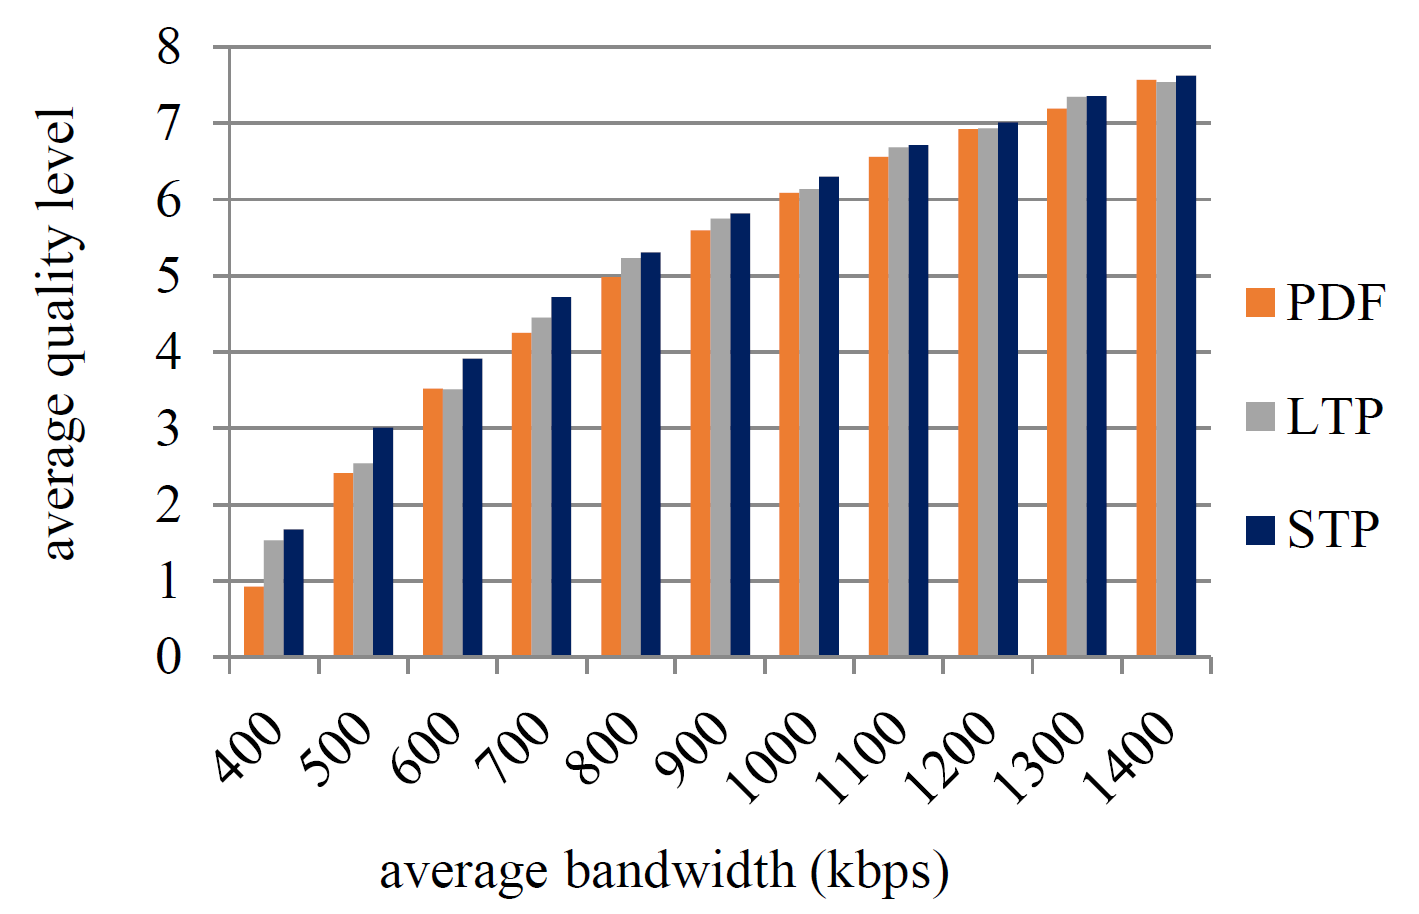
\includegraphics[width=0.40\textwidth]{Quality-all.png}
\label{fig:quality-all}}
\subfloat[Quality level variance of different control algorithms]{
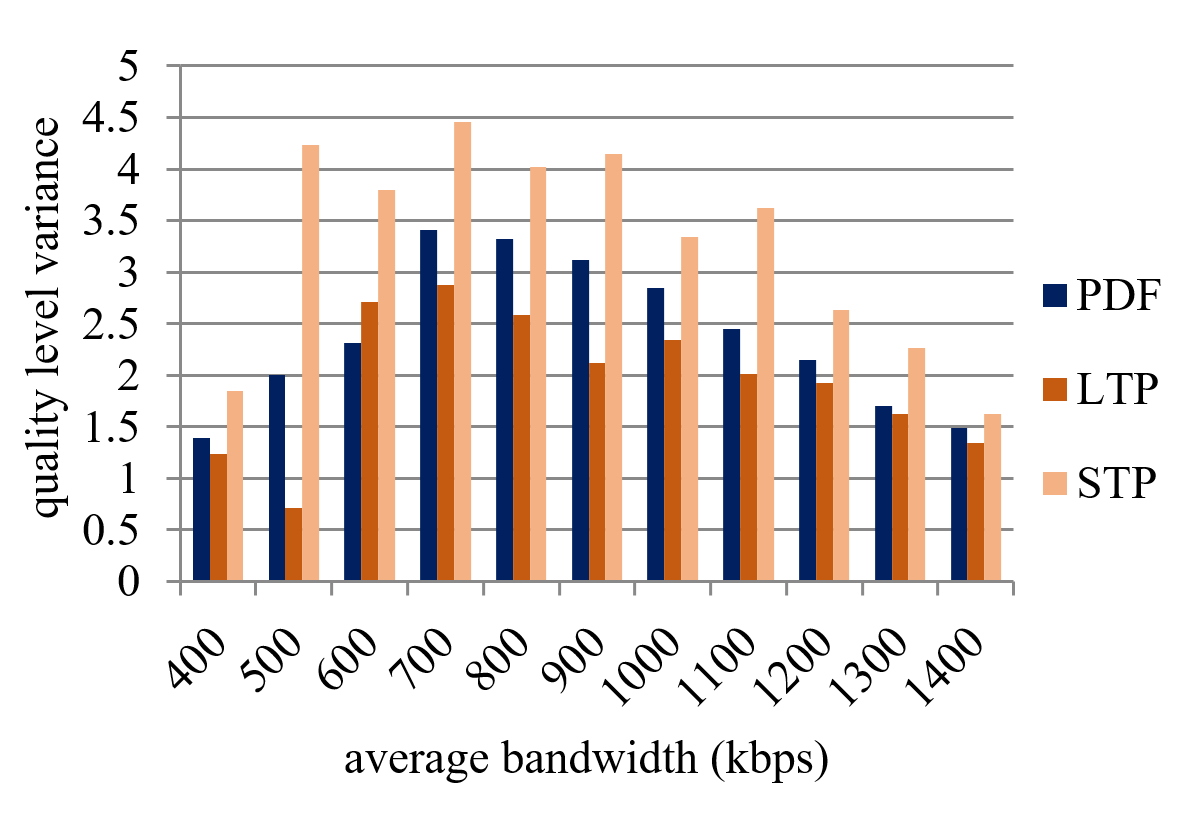
\includegraphics[width=0.40\textwidth]{Variance-all.png}
\label{fig:variance-all}}
\caption{Comparison of the long/short time prediction and the PDF algorithm in DSS}
\label{fig:performance-all}
\end{figure*}

\begin{figure*}[t]
\centering
\subfloat[Average quality level of the PID and PDF control algorithms]{
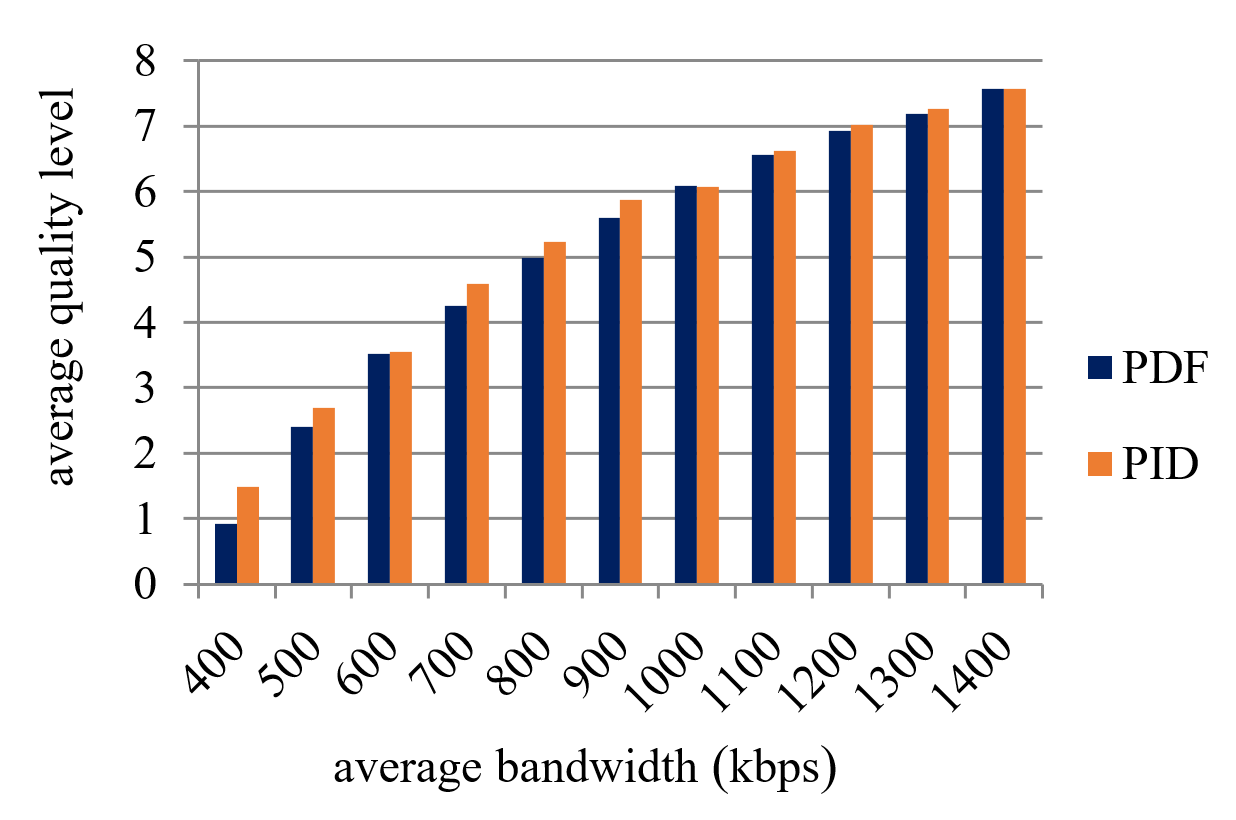
\includegraphics[width=0.40\textwidth]{Quality-two.png}
\label{fig:quality-two}}
\subfloat[Quality level variance of the PID and PDF control algorithms]{
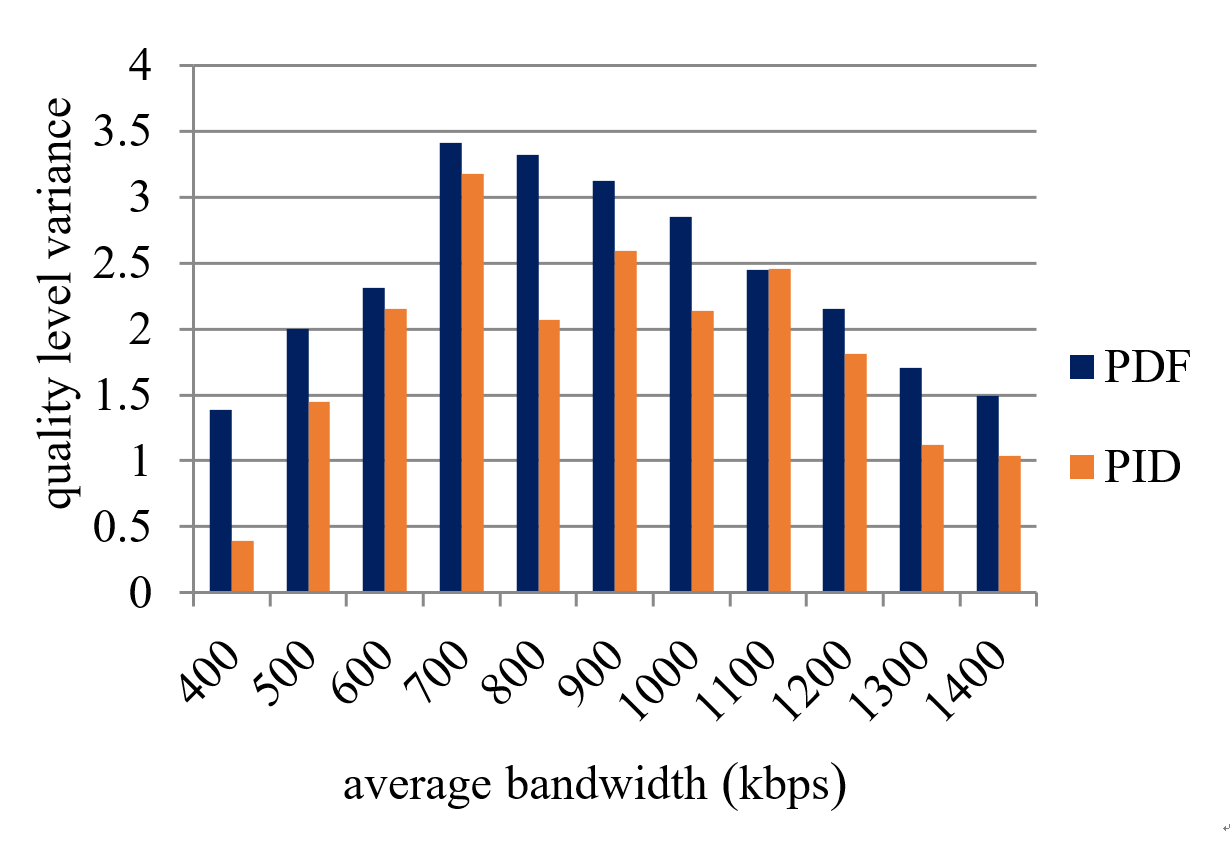
\includegraphics[width=0.40\textwidth]{Variance-two.png}
\label{fig:variance-two}}
\caption{Comparison of the proposed PID algorithm and the PDF algorithm in DDS}
\label{fig:performance-two}
\end{figure*}

\begin{table*}[t]
\centering
\caption{Improvement of different quality control algorithms}
\label{tab:improvement}
\begin{tabular}[b]{p{4.2cm}<{\centering}|p{4.2cm}<{\centering}|p{4.2cm}<{\centering}}
\hline \hline
Quality control algorithm & Average quality level & Quality variance \\ \hline
Packet delay feedback (PDF) & 0.0\% & 0.0\% \\ \hline
Short term prediction (STP) & \textbf{+13.5\%} & +38.5\% \\ \hline
Long term prediction (LTP) & +7.9\% & -17.2\% \\ \hline
PID based control scheme(PID) & +8.6\% & \textbf{-24.8\%} \\ \hline
\end{tabular}
\end{table*}

Since STP and LTP have their own limitations, we implement the complete PID-based quality control algorithm, which can both reduce the quality variance and improve the average quality level. From the results shown in Fig. \ref{fig:performance-two}, we can conclude that when integrated with the integral part and the derivative part, the effect of the proportional part is not as aggressive as that in STP. An obvious proof can be found in Fig. \ref{fig:variance-two}, which clearly shows that the proposed PID quality control algorithm achieves a lower quality variance compared to the PDF algorithm. Table \ref{tab:improvement} lists the statistical experimental results for these four quality control algorithms, in which the PID-based control algorithm has shown its advantage over the others, especially in reducing the quality fluctuation. It can be seen that, compared to PDF, the PID-based quality control algorithm improves 8.6\% in video quality with a 24.8\% reduction in quality fluctuation. The video quality fluctuation of the four control algorithms, when the bandwidth fluctuates around 800 kbps, is shown in Fig. \ref{fig:fluctuation}, from which we can observe a more stable video quality in the proposed PID quality control algorithm.

\begin{figure}
\centering
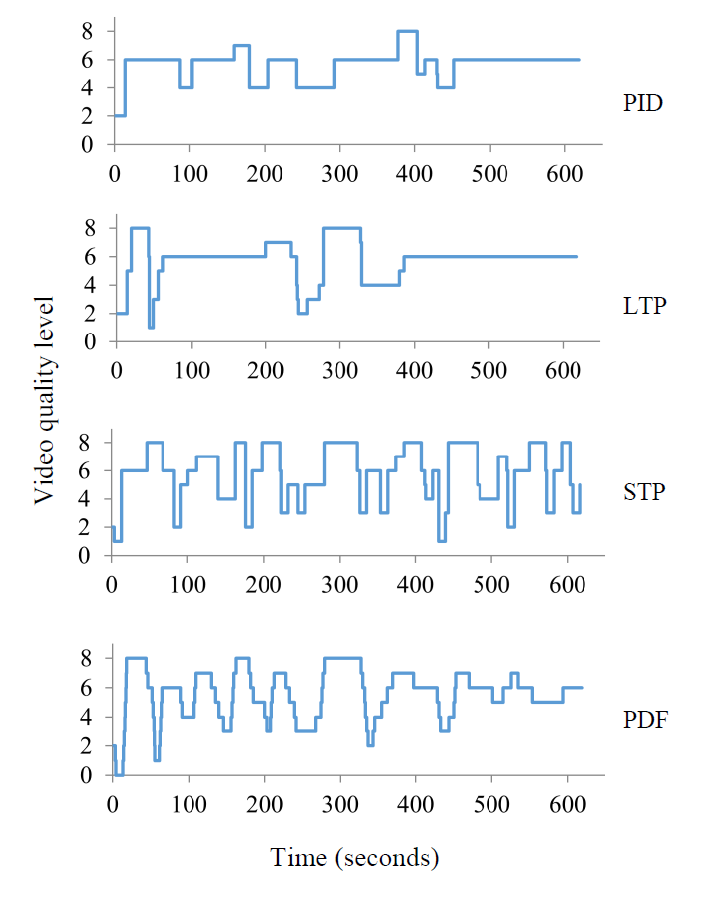
\includegraphics[width = 0.8\linewidth]{Fluctuation.png}
\caption{Video quality fluctuation with time \label{fig:fluctuation}}
\end{figure}

\subsection{Results of the Combined System}
\label{subsec:exp-combined}

After combining the two algorithms together, the proposed adaptive streaming system is able to deliver a higher and smoother video quality for the user. The system works as follows. The greedy-like algorithm present in \ref{subsec:priority-assign} is performed first to determine the priority values for all enhancement NALUs in an SVC bitstream. Then, the priority values are injected into the bitstream and stored in the priority identifier field of the NALU header. When DSS streams this video, it can extract an optimized sub-stream by simply checking this field and discarding the packets with lower priority values. The bitrate of the sub-stream to be extracted is determined by the PID-based quality control algorithm according to the network condition.

We compare the combined system's performance with DSS that supports SVC but uses its original quality control method and the JSVM Basic bitstream extraction. The result for the test sequence Soccer is presented in Fig. \ref{fig:fluctuation-psnr}, which shows the change of the streamed video's PSNR when the available bandwidth fluctuates around 400 kbps, 600 kbps, 800 kbps and 1000 kbps (bandwidth fluctuation is simulated the same way as in the previous experiments). It can be seen that, the proposed system performs better in that it has effectively avoided unnecessary quality drops (e.g., note the curve around time 350 s in Fig. \ref{fig:Fluctuation-PSNR3} or 150 s in Fig. \ref{fig:Fluctuation-PSNR4}) and is able to keep a relatively higher PSNR value (e.g., note the curve around time 450 s in Fig. \ref{fig:Fluctuation-PSNR1} or 500 s in Fig. \ref{fig:Fluctuation-PSNR2}). The average and variance of the PSNR through the time are also calculated and presented in Fig. \ref{fig:fluctuation-psnr}, showing clearly the proposed system's advantage. For instance, in Fig. \ref{fig:Fluctuation-PSNR3} where the bandwidth fluctuates around 800 kbps, the average PSNR delivered by the proposed system is 38.75 dB, 0.83 dB higher than that of the baseline system, and the PSNR variance is also reduced from 1.24 to 0.69, indicating a smoother video quality change.

\begin{figure*}[t]
\centering
\subfloat[Bandwidth fluctuates around 400 kbps: the PSNR average and variance in the original system are 36.00 and 0.30, while in the proposed system are 36.50 (increased by 0.50) and 0.23 (reduced by 0.07).]{
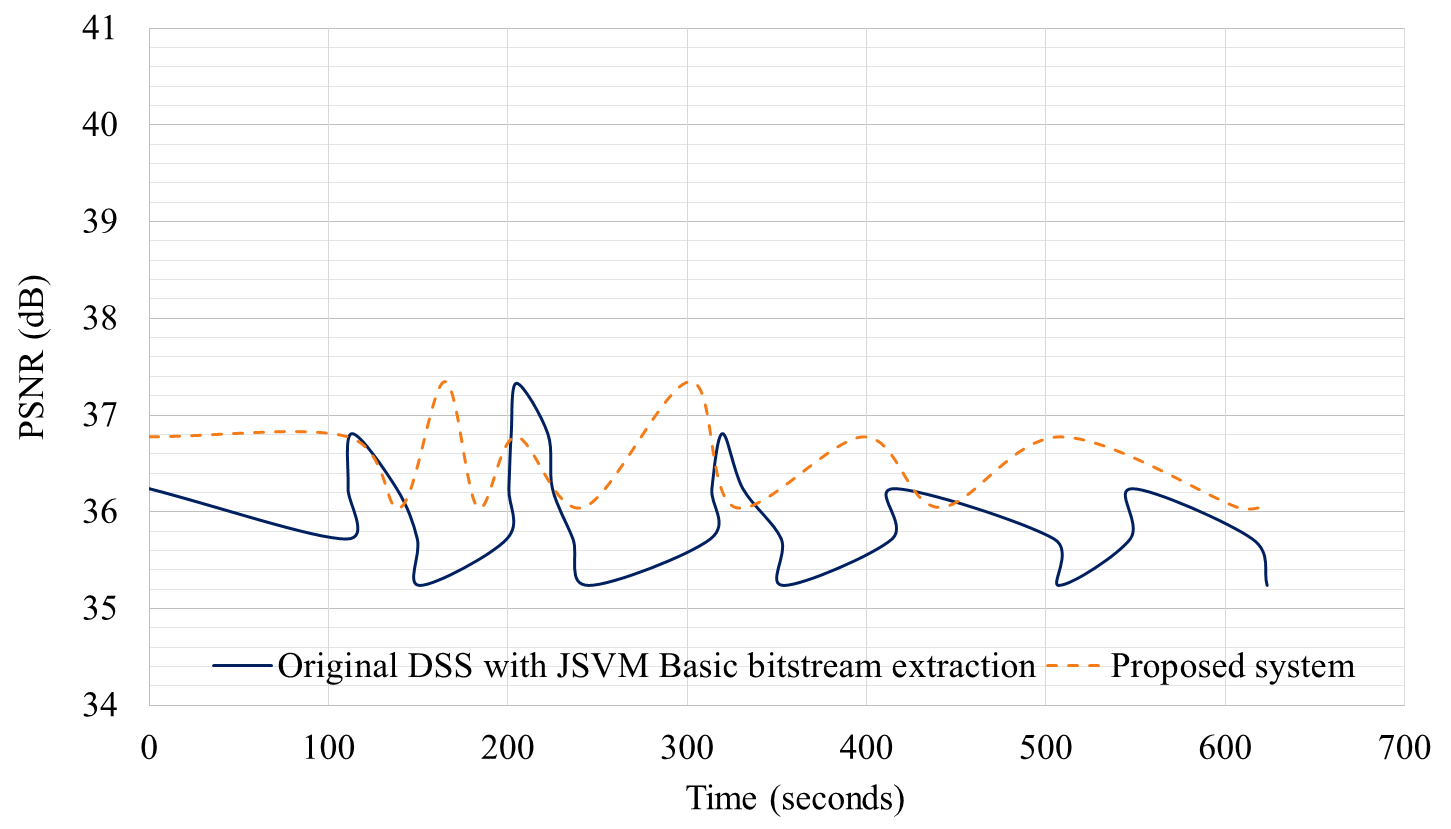
\includegraphics[width=0.45\textwidth]{Fluctuation-PSNR1.png}
\label{fig:Fluctuation-PSNR1}}\hfill
\subfloat[Bandwidth fluctuates around 600 kbps: the PSNR average and variance in the original system are 37.06 and 0.61, while in the proposed system are 37.32 (increased by 0.26) and 0.33 (reduced by 0.28).]{
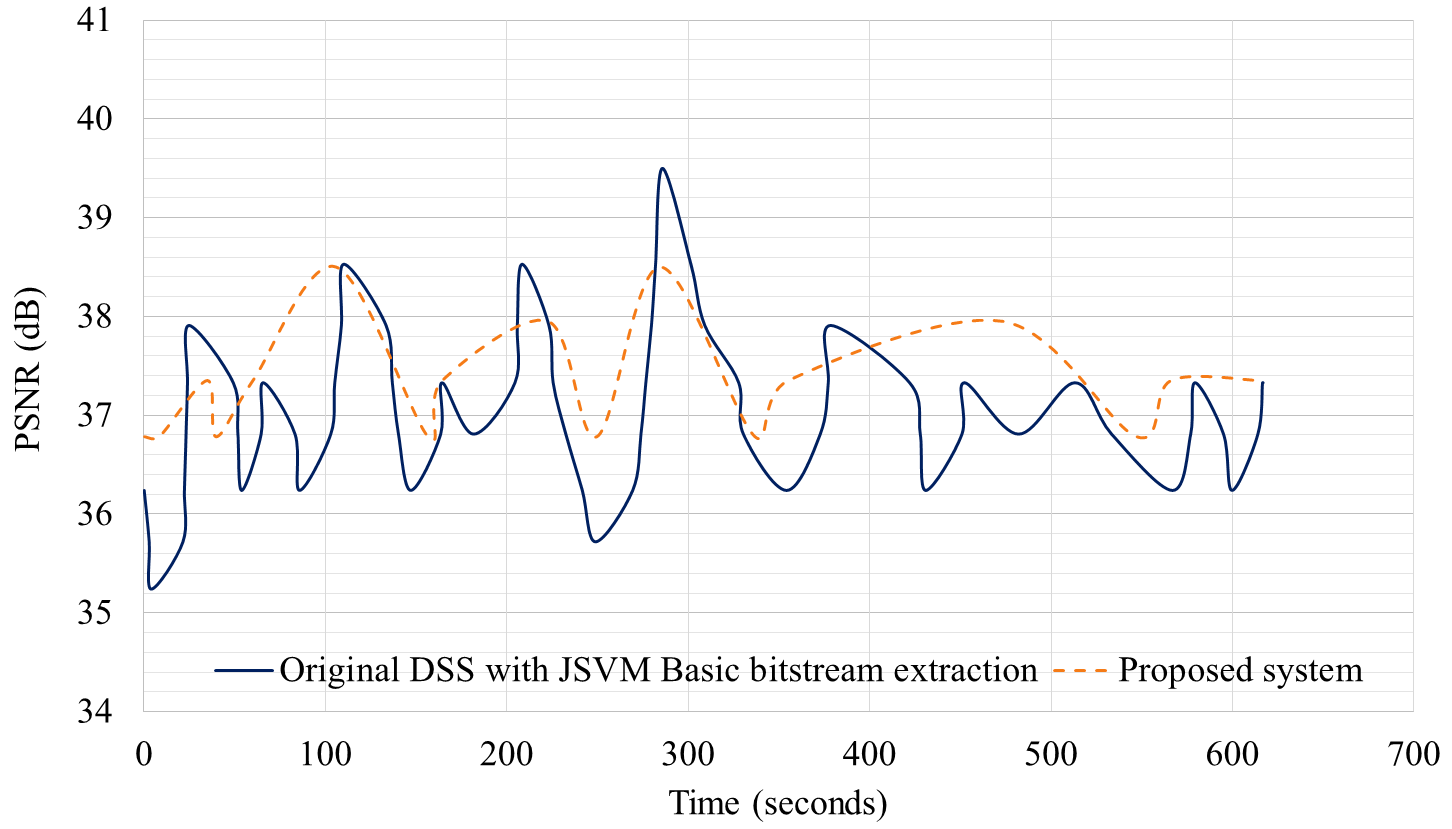
\includegraphics[width=0.45\textwidth]{Fluctuation-PSNR2.png}
\label{fig:Fluctuation-PSNR2}}
\qquad
\subfloat[Bandwidth fluctuates around 800 kbps: the PSNR average and variance in the original system are 37.92 and 1.24, while in the proposed system are 38.75 (increased by 0.83) and 0.69 (reduced by 0.55).]{
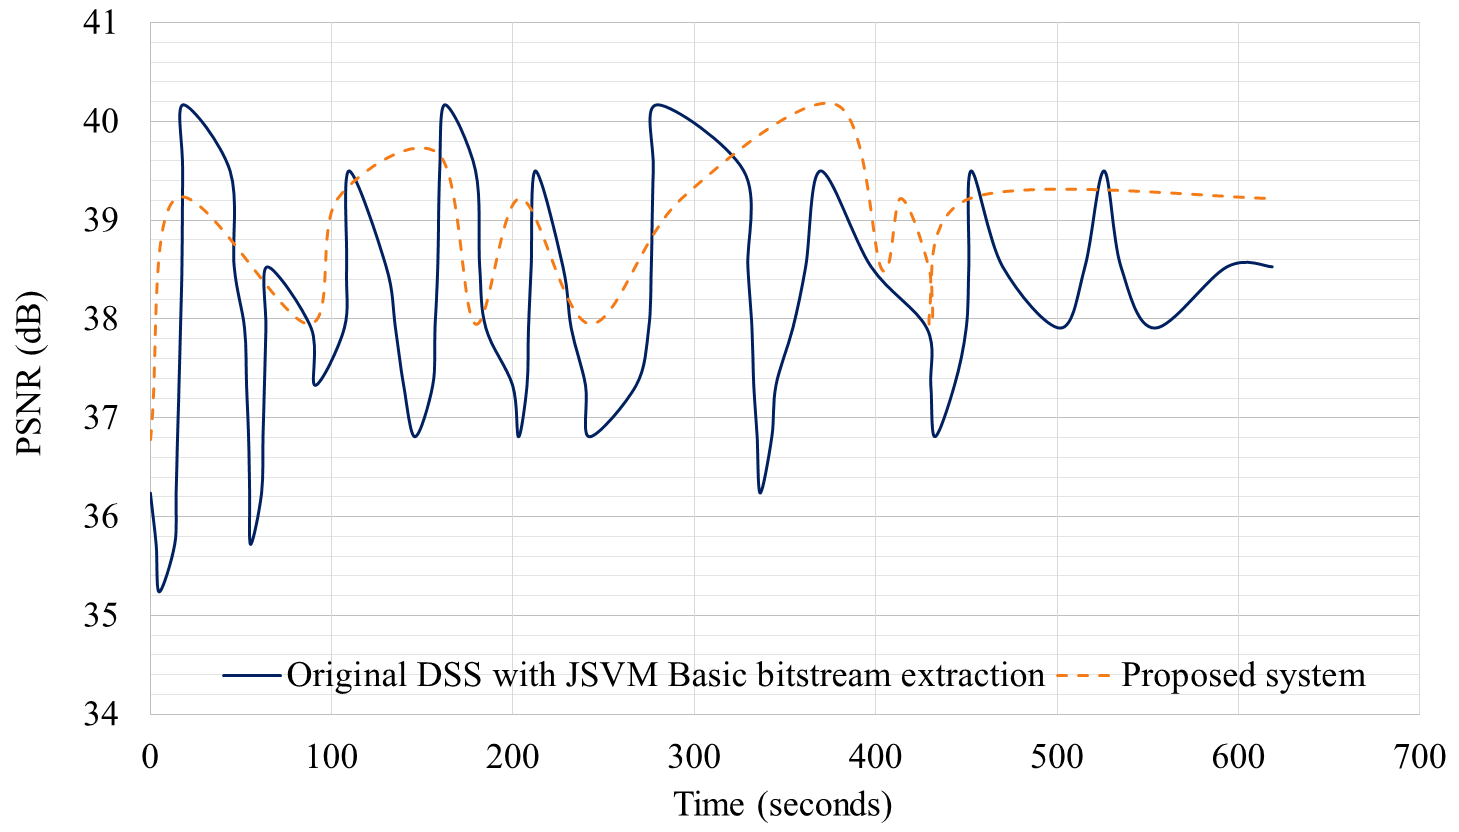
\includegraphics[width=0.45\textwidth]{Fluctuation-PSNR3.png}
\label{fig:Fluctuation-PSNR3}}\hfill
\subfloat[Bandwidth fluctuates around 1000 kbps: the PSNR average and variance in the original system are 38.28 and 1.30, while in the proposed system are 38.94 (increased by 0.66) and 0.71 (reduced by 0.59).]{
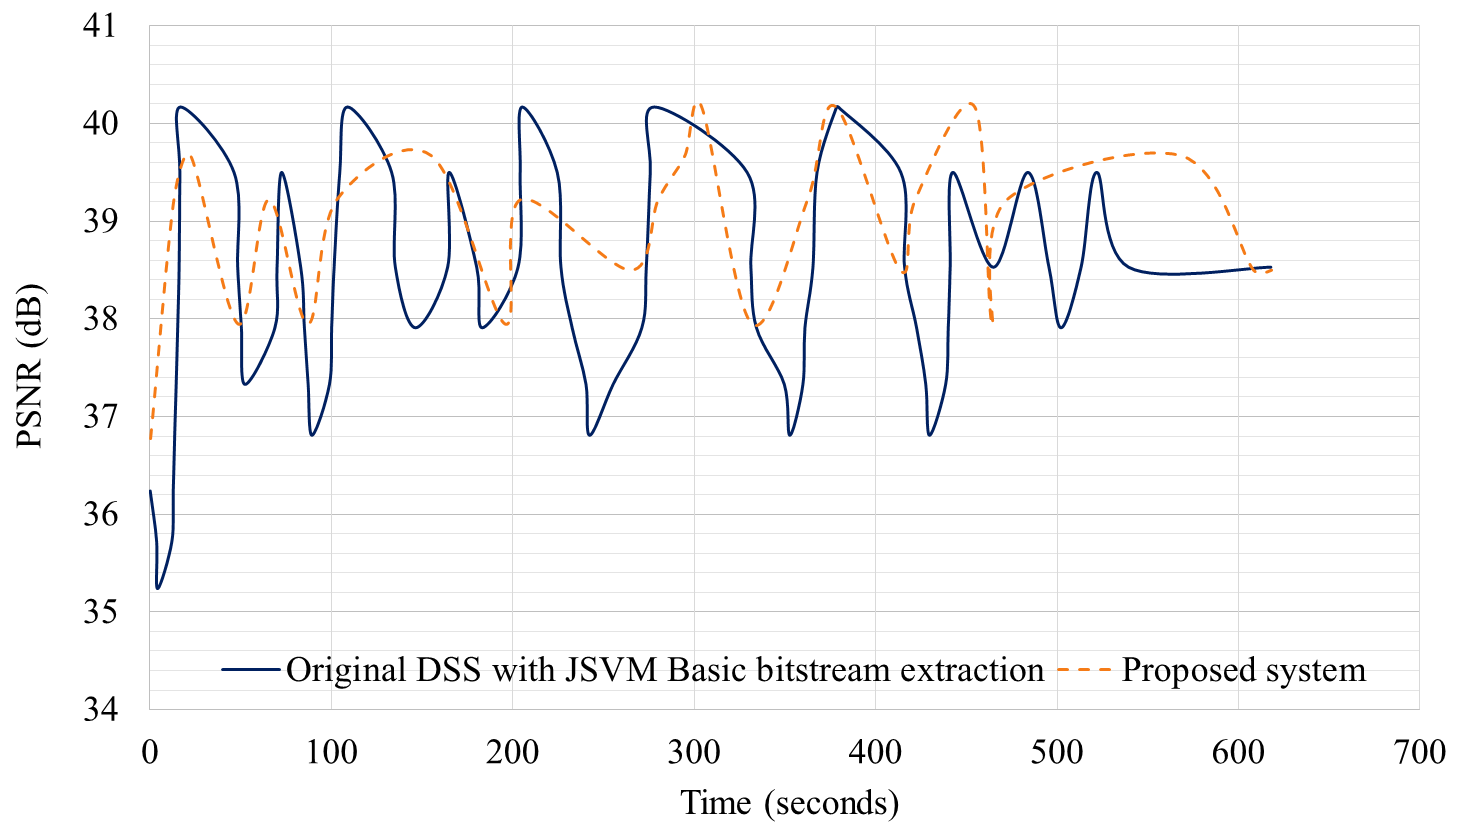
\includegraphics[width=0.45\textwidth]{Fluctuation-PSNR4.png}
\label{fig:Fluctuation-PSNR4}}
\caption{Change of the streamed video's PSNR during bandwidth fluctuation
\label{fig:fluctuation-psnr}}
\end{figure*}

\section{Conclusion}
\label{sec:conclusion}

In this paper, an adaptive video streaming system with optimized bitstream extraction and PID-based quality control is proposed. The bitstream extraction method includes a linear error model to estimate the distortion caused by discarding any combination of packets and a greedy algorithm to assign priority to each data packet. The priority values can then be stored in the bitstream and used for R-D optimized extraction. Experimental results show that the method can achieve PSNR gain of up to 0.5 dB compared to the JSVM QL extractor under the same bitrate constraint, also with the same computational complexity. The PID-based quality control algorithm has a flexible mechanism to determine the suitable quality level for transmission so that it provides an accurate and swift response to the bandwidth change. Compared to the original algorithm in DSS, this algorithm has reduced quality fluctuation significantly to improve audience satisfaction. The proposed SVC adaptive streaming system integrated with these two solutions performs well in terms of automatically adapting to the user's bandwidth fluctuation, and it is able to provide the user a better watching experience.

Because the next-generation video coding standard High Efficiency Video Coding (HEVC) \cite{HEVC} adopts the same coding framework as its predecessor H.264/AVC, we expect to apply this paper's model and approach of bitstream extraction to the emerging HEVC standard and its scalable extension. As for the PID-based quality control algorithm, it is only network-concerned and thus should be easily integrated into other streaming systems, e.g., a simulcast system such as DASH. Another direction for future work is to carry out some subjective tests, demonstrating the performance of the proposed system from the perceived quality point of view.

% Can use something like this to put references on a page
% by themselves when using endfloat and the captionsoff option.
\ifCLASSOPTIONcaptionsoff
  \newpage
\fi



% trigger a \newpage just before the given reference
% number - used to balance the columns on the last page
% adjust value as needed - may need to be readjusted if
% the document is modified later
%\IEEEtriggeratref{8}
% The "triggered" command can be changed if desired:
%\IEEEtriggercmd{\enlargethispage{-5in}}

% references section

% can use a bibliography generated by BibTeX as a .bbl file
% BibTeX documentation can be easily obtained at:
% http://www.ctan.org/tex-archive/biblio/bibtex/contrib/doc/
% The IEEEtran BibTeX style support page is at:
% http://www.michaelshell.org/tex/ieeetran/bibtex/
%\bibliographystyle{IEEEtran}
% argument is your BibTeX string definitions and bibliography database(s)
%\bibliography{IEEEabrv,../bib/paper}
%
% <OR> manually copy in the resultant .bbl file
% set second argument of \begin to the number of references
% (used to reserve space for the reference number labels box)
\begin{thebibliography}{1}

\bibitem{Gualdi08}
G. Gualdi, A. Prati, and R. Cucchiara, ``Video Streaming for Mobile Video Surveillance'', {\em IEEE Transactions on Multimedia}, vol. 10, no. 6, pp. 1142-1154, 2008.

\bibitem{Chen13}
Y. Chen, B. Zhang, Y. Liu, and W. Zhu, ``Measurement and Modeling of Video Watching Time in a Large-Scale Internet Video-on-Demand System'', {\em IEEE Transactions on Multimedia}, vol. 15, no. 8, pp. 2087-2098, 2013.

\bibitem{Egilmez14}
H. E. Egilmez and A. M. Tekalp, ``Distributed QoS architectures for multimedia streaming over software defined networks'', {\em IEEE Transactions on Multimedia}, vol. 16, no. 6, pp. 1597-1609, 2014.

\bibitem{Li14}
S. Li et al., ``Flexible Traffic Engineering (F-TE): When OpenFlow Meets Multi-Protocol IP-Forwarding'', {\em IEEE Communication Letters}, vol. 18, pp. 1699-1702, Oct. 2014.

\bibitem{Xue15}
N. Xue et al., ``Demonstration of OpenFlow-Controlled Network Orchestration for Adaptive SVC Video Manycast'', {\em IEEE Transactions on Multimedia}, vol. 17, pp. 1617-1629, Sept. 2015.

\bibitem{DASH}
T. Stockhammer, ``Dynamic adaptive streaming over HTTP: standards and design principles'', {\em Proceedings of the second annual ACM conference on Multimedia systems}, 2011.

\bibitem{SVC}
T.~Wiegand, G.~Sullivan, J.~Reichel, H.~Schwarz, M.~Wien, eds., ``Joint Draft ITU-T Rec. H.264|ISO/IEC 14496-10/Amd.3 Scalable Video Coding'', Joint Video Team, Doc. JVT-X201 Jul. 2007.

\bibitem{SVCOverview}
H.~Schwarz, D.~Marpe, and T.~Wiegand, ``Overview of the scalable video coding extension of the H.264/AVC standard'', {\em IEEE Trans. Circuits. Syst. Video Technol.}, vol. 17, no. 9, pp. 1103-1120, 2007.

\bibitem{Bouten14}
N. Bouten, S. Latre, J. Famaey, W. V. Leekwijck, and F. D. Turck, ``In-Network Quality Optimization for Adaptive Video Streaming Services'', {\em IEEE Transactions on Multimedia}, vol. 16, no. 8, pp. 2281-2293, 2014.

\bibitem{YouTube}
https://www.youtube.com/

\bibitem{SVCPerformance}
M. Wien , H. Schwarz and T. Oelbaum,  ``Performance Analysis of SVC'', {\em IEEE Trans. Circuits Syst. Video Technol.}, vol. 17, no. 9, pp. 1194-1203, 2007.

\bibitem{Chuah12}
S. Chuah, Z. Chen, and Y. Tan, ``Energy-Efficient Resource Allocation and Scheduling for Multicast of Scalable Video Over Wireless Networks'', {\em IEEE Transactions on Multimedia}, vol. 14, no. 4, pp. 1324-1336, 2012.

\bibitem{Zhu13}
Z. Zhu, S. Li, and X. Chen, ``Design QoS-aware multi-path provisioning strategies for efficient cloud-assisted SVC video streaming to heterogeneous clients'', {\em IEEE Transactions on Multimedia}, vol. 15, no. 4, pp. 758-768, 2013.

\bibitem{Dan13}
G. Dan, O. Hadar, R. Ohayon, and N. Amram, ``Live video streaming with adaptive pre-processing by using scalable video coding'', {\em Proceedings of IEEE International Conference on Consumer Electronics (ICCE)}, pp. 588-589, 2013.

\bibitem{Yang14}
E. Yang, Y. Ran, S. Chen, and J. Yang, ``A multicast architecture of SVC streaming over OpenFlow networks'', {\em Proceedings of IEEE Global Communications Conference (GLOBECOM)}, pp. 1323-1328, 2014.

\bibitem{Cicalo14}
S. Cicalo, and V. Tralli, ``Distortion-Fair Cross-Layer Resource Allocation for Scalable Video Transmission in OFDMA Wireless Networks'', {\em IEEE Transactions on Multimedia}, vol. 16, no. 3, pp. 848-863, 2014.

\bibitem{DSS}
http://dss.macosforge.org/

\bibitem{Knapsack}
http://en.wikipedia.org/wiki/Knapsack\_problem

\bibitem{Amonou07}
I.~Amonou, N.~Cammas, S.~Kervadec, S.~Pateux, ``Optimized Rate-distortion Extraction with Quality Layers in the Scalable Extension of H.264/AVC'', {\em IEEE Trans. Circuits Syst. Video Technol.}, vol. 17, no. 9, pp. 1186-1193, 2007.

\bibitem{JSVM}
Text of ISO/IEC 14496-4:2001/PDAM 19 Reference Software for SVC, Joint Video Team (JVT) of ISO-IEC MPEG \& ITU-T VCEG, N9195, Sep. 2007.

\bibitem{Sun09}
J.~Sun, W.~Gao, D.~Zhao, W.~Li, ``On Rate-distortion Modeling and Extraction of H.264/SVC Fine-Granular Scalable Video'', {\em IEEE Trans. Circuits Syst. Video Technol.}, vol.~19, no.~3, pp.~323-336, Mar. 2009.

\bibitem{Maani09}
E.~Maani, A.~K. Katsaggelos, ``Optimized Bit Extraction Using Distortion Modeling in the Scalable Extension of H.264/AVC'', {\em IEEE Trans. Image Processing}, vol.~18, no.~9, pp.~2022-2029, 2009.

\bibitem{Ramanathan12}
P.~Ramanathan and N.~Jayant. ``RD optimized bitstream extraction for H. 264/SVC based video streaming'', {\em Proceedings of IEEE International Conference on Image Processing}, pp. 2241-2244, 2012.

\bibitem{Yang13}
K.~Yang, S.~Wan, Y.~Gong, and Y.~Feng. ``A fast algorithm of bitstream extraction using distortion prediction based on simulated annealing'', {\em Journal of Visual Communication and Image Representation}, no.7, pp. 752-759, 2013.

\bibitem{Lim06}
J. Lim, M. Kin, and S. Hahm, ``An optimization-theoretic approach to optimal extraction of SVC Bitstreams'', ITU-T VCEG
JVT-U081, October 2006.

\bibitem{Zhu11}
T. Zhu and X. Zhang, ``Frame distortion estimation and its application to extraction priority assignment for MGS of H. 264/SVC'', {\em Przegląd Elektrotechniczny}, vol. 87, no. 1, pp. 284-289, 2011.

\bibitem{Zhang12}
W.~Zhang, J.~Sun, J.~Liu and Z.~Guo, ``Optimized bit extraction of SVC exploiting linear error model'', {\em Proceedings of IEEE International Symposium on Circuits and Systems}, pp.~1887-1890, Seoul, Korea, May 2012.

\bibitem{Gao06}
K. Gao, J. Zhai, J. Li and C. Wang, ``Real-Time scheduling for scalable video coding streaming system'', {\em IEEE Sarnoff Symposium}, Princeton, NJ, pp. 1-4, Mar. 2006.

\bibitem{Schierl10}
Y. Schierl, R. Sanchez, C. Globisch, Hellge, and T. Wiegand, ``Priority-based media delivery using SVC with RTP and HTTP streaming'', {\em Multimedia Tools And Applications}, vol. 55, no. 2, pp. 227-246, Sep. 2010.

\bibitem{Winken08}
M.~Winken, H.~Schwarz, T.~Wiegand, ``Joint Rate-distortion Optimization of Transform Coefficients for Spatial Scalable Video Coding Using SVC'', {\em Proceedings of IEEE International Conference on Image Processing}, 2008.

\bibitem{H264Overview}
T.~Wiegand, G.~J. Sullivan, G.~Bj$\o$ntegaard, A.~Luthra, ``Overview of the H.264/AVC Video Coding Standard'', {\em IEEE Trans. Circuits Syst. Video Technol.}, vol. 13, no. 7, pp.~560--576, Jul. 2003.

\bibitem{GreedyAlgo}
P.~E.~Black, ``Greedy Algorithm'' in {\em Dictionary of Algorithms and Data Structures} [online], U.S. National Institute of Standards and Technology, Feb. 2005.
\newblock http://www.nist.gov/dads/HTML/greedyalgo.html

\bibitem{PID}
http://en.wikipedia.org/wiki/PID\_controller

\bibitem{Astrom02}
K. J. Astrom, Control System Design, pp 216-219, 2002.

\bibitem{Wong04}
C.W.Wong, O.C.Au and H.K.Lam, ``PID-based real-time rate control'', {\em Proceedings of IEEE International Conference on Multimedia and Expo}, 1: 221-224, 2004.

\bibitem{Li98}
B. Li and K. Nahrstedt  ``A control theoretical model for quality of service adaptations'', {\em Proceedings of Sixth International Workshop on Quality of Service}, 1998.

\bibitem{Li99}
B. Li and K. Nahrstedt, ``A control-sased middleware framework for Quality-of-Service adaptations'', {\em IEEE J. Selected Areas in Comm.}, vol. 17, no. 9, pp. 1632-1650, Sept. 1999.

\bibitem{Ziegler42}
J. B. Ziegler and N. B. Nichols, ``Optimum settings for automatic controllers'', {\em ASME Trans.}, pp. 759-768, 1942.

\bibitem{Netlimiter}
NetLimiter: http://www.netlimiter.com/

\bibitem{HEVC}
G.~J.~Sullivan, J.-R.~Ohm, W.-J.~Han, and T.~Wiegand, ``Overview of the High Efficiency Video Coding (HEVC) standard'', {\em IEEE Trans. Circuits Syst. Video Technol.}, vol.~22, no.~12, pp.~1648-1667, Dec. 2012. 

\end{thebibliography}



% biography section
% 
% If you have an EPS/PDF photo (graphicx package needed) extra braces are
% needed around the contents of the optional argument to biography to prevent
% the LaTeX parser from getting confused when it sees the complicated
% \includegraphics command within an optional argument. (You could create
% your own custom macro containing the \includegraphics command to make things
% simpler here.)

\begin{IEEEbiography}[{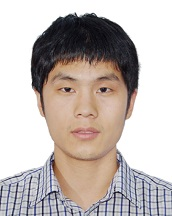
\includegraphics[width=1in,height=1.25in,clip,keepaspectratio]{ShengbinMeng.jpg}}]{Shengbin Meng}
received the B.E. degree in automation engineering from Tsinghua University, Beijing, China, in 2011. He is currently working towards the Ph.D. degree in computer science at the Institute of Computer Science and Technology, Peking University, Beijing, China.

His current research interests include video coding, codec implementation and optimization, video streaming, and multimedia applications.
\end{IEEEbiography}

\begin{IEEEbiography}[{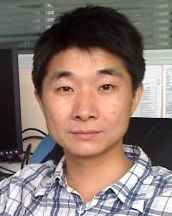
\includegraphics[width=1in,height=1.25in,clip,keepaspectratio]{JunSun.jpg}}]{Jun Sun}
(M’07) received the B.S. degree in computer science from the University of Science and Technology Beijing, Beijing, China, in 1999, and the Ph.D. degree in computer science from the Institute of Computing Technology, Chinese Academy of Sciences, Beijing, China, in 2006.

From 2006 to 2008, he was a Post-Doctorate with the Institute of DigitalMedia, EECS, Peking University, Beijing, China. He then joined the Institute of Computer Science and Technology, Peking University, Beijing, China, where he is currently an Associate Professor. His research interests include scalable video coding, rate-distortion analysis, video transcoding, video streaming, and video scheduling in wireless networks. He has published over 30 technical articles in referred journals and proceedings in the areas of video coding and analysis.
\end{IEEEbiography}

\begin{IEEEbiography}[{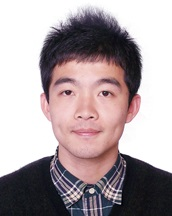
\includegraphics[width=1in,height=1.25in,clip,keepaspectratio]{YizhouDuan.jpg}}]{Yizhou Duan}
received the B.S. degree and the Ph.D degree in computer science from Peking University, Beijing, China, in 2009 and 2015, respectively. He is currently working for Strongene Ltd., Beijing, China.

His current research interests include video coding, codec implementation and optimization, scalable video systems, and rate-distortion analysis.
\end{IEEEbiography}

\begin{IEEEbiography}[{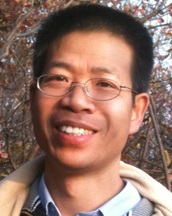
\includegraphics[width=1in,height=1.25in,clip,keepaspectratio]{ZongmingGuo.jpg}}]{Zongming Guo}
(M’09) received the B.S. degree in mathematics, and the M.S. and Ph.D. degrees in computer science from Peking University, Beijing, China, in 1987, 1990, and 1994, respectively.

He is currently a Professor with the Institute of Computer Science and Technology, Peking University. His current research interests include video coding, processing, and communication.

Dr. Guo is the Executive Member of the China-Society of Motion Picture and Television Engineers. He was a recipient of the First Prize of the State Administration of Radio Film and Television Award in 2004, the First Prize of the Ministry of Education Science and Technology Progress Award in 2006, the Second Prize of the National Science and Technology Award in 2007, the Wang Xuan News Technology Award and the Chia Tai Teaching Award in 2008, the Government Allowance granted by the State Council in 2009, and the Distinguished Doctoral Dissertation Advisor Award of Peking University in 2012 and 2013.

\end{IEEEbiography}

% if you will not have a photo at all:
%\begin{IEEEbiographynophoto}{John Doe}
%Biography text here.
%\end{IEEEbiographynophoto}

% insert where needed to balance the two columns on the last page with
% biographies
%\newpage

% You can push biographies down or up by placing
% a \vfill before or after them. The appropriate
% use of \vfill depends on what kind of text is
% on the last page and whether or not the columns
% are being equalized.

%\vfill

% Can be used to pull up biographies so that the bottom of the last one
% is flush with the other column.
%\enlargethispage{-5in}

% that's all folks
\end{document}


